\chapter{Prezentacja projektu}
Rozdział zawiera zdjęcie i opisy przedstawiające działanie aplikacji mobilnej i strony internetowej.

\section{Strona internetowa}
Rozdział przedstawia widoki i działanie strony internetowej.

\subsection{Logowanie}
Po uruchomieniu strony ukazuje się widok zawierający formularz logowania do strony internetowej. Po pomyślnym zalogowaniu użytkownik zostaje przekierowany do strony domowej.


\begin{figure}[H]
    \centering
    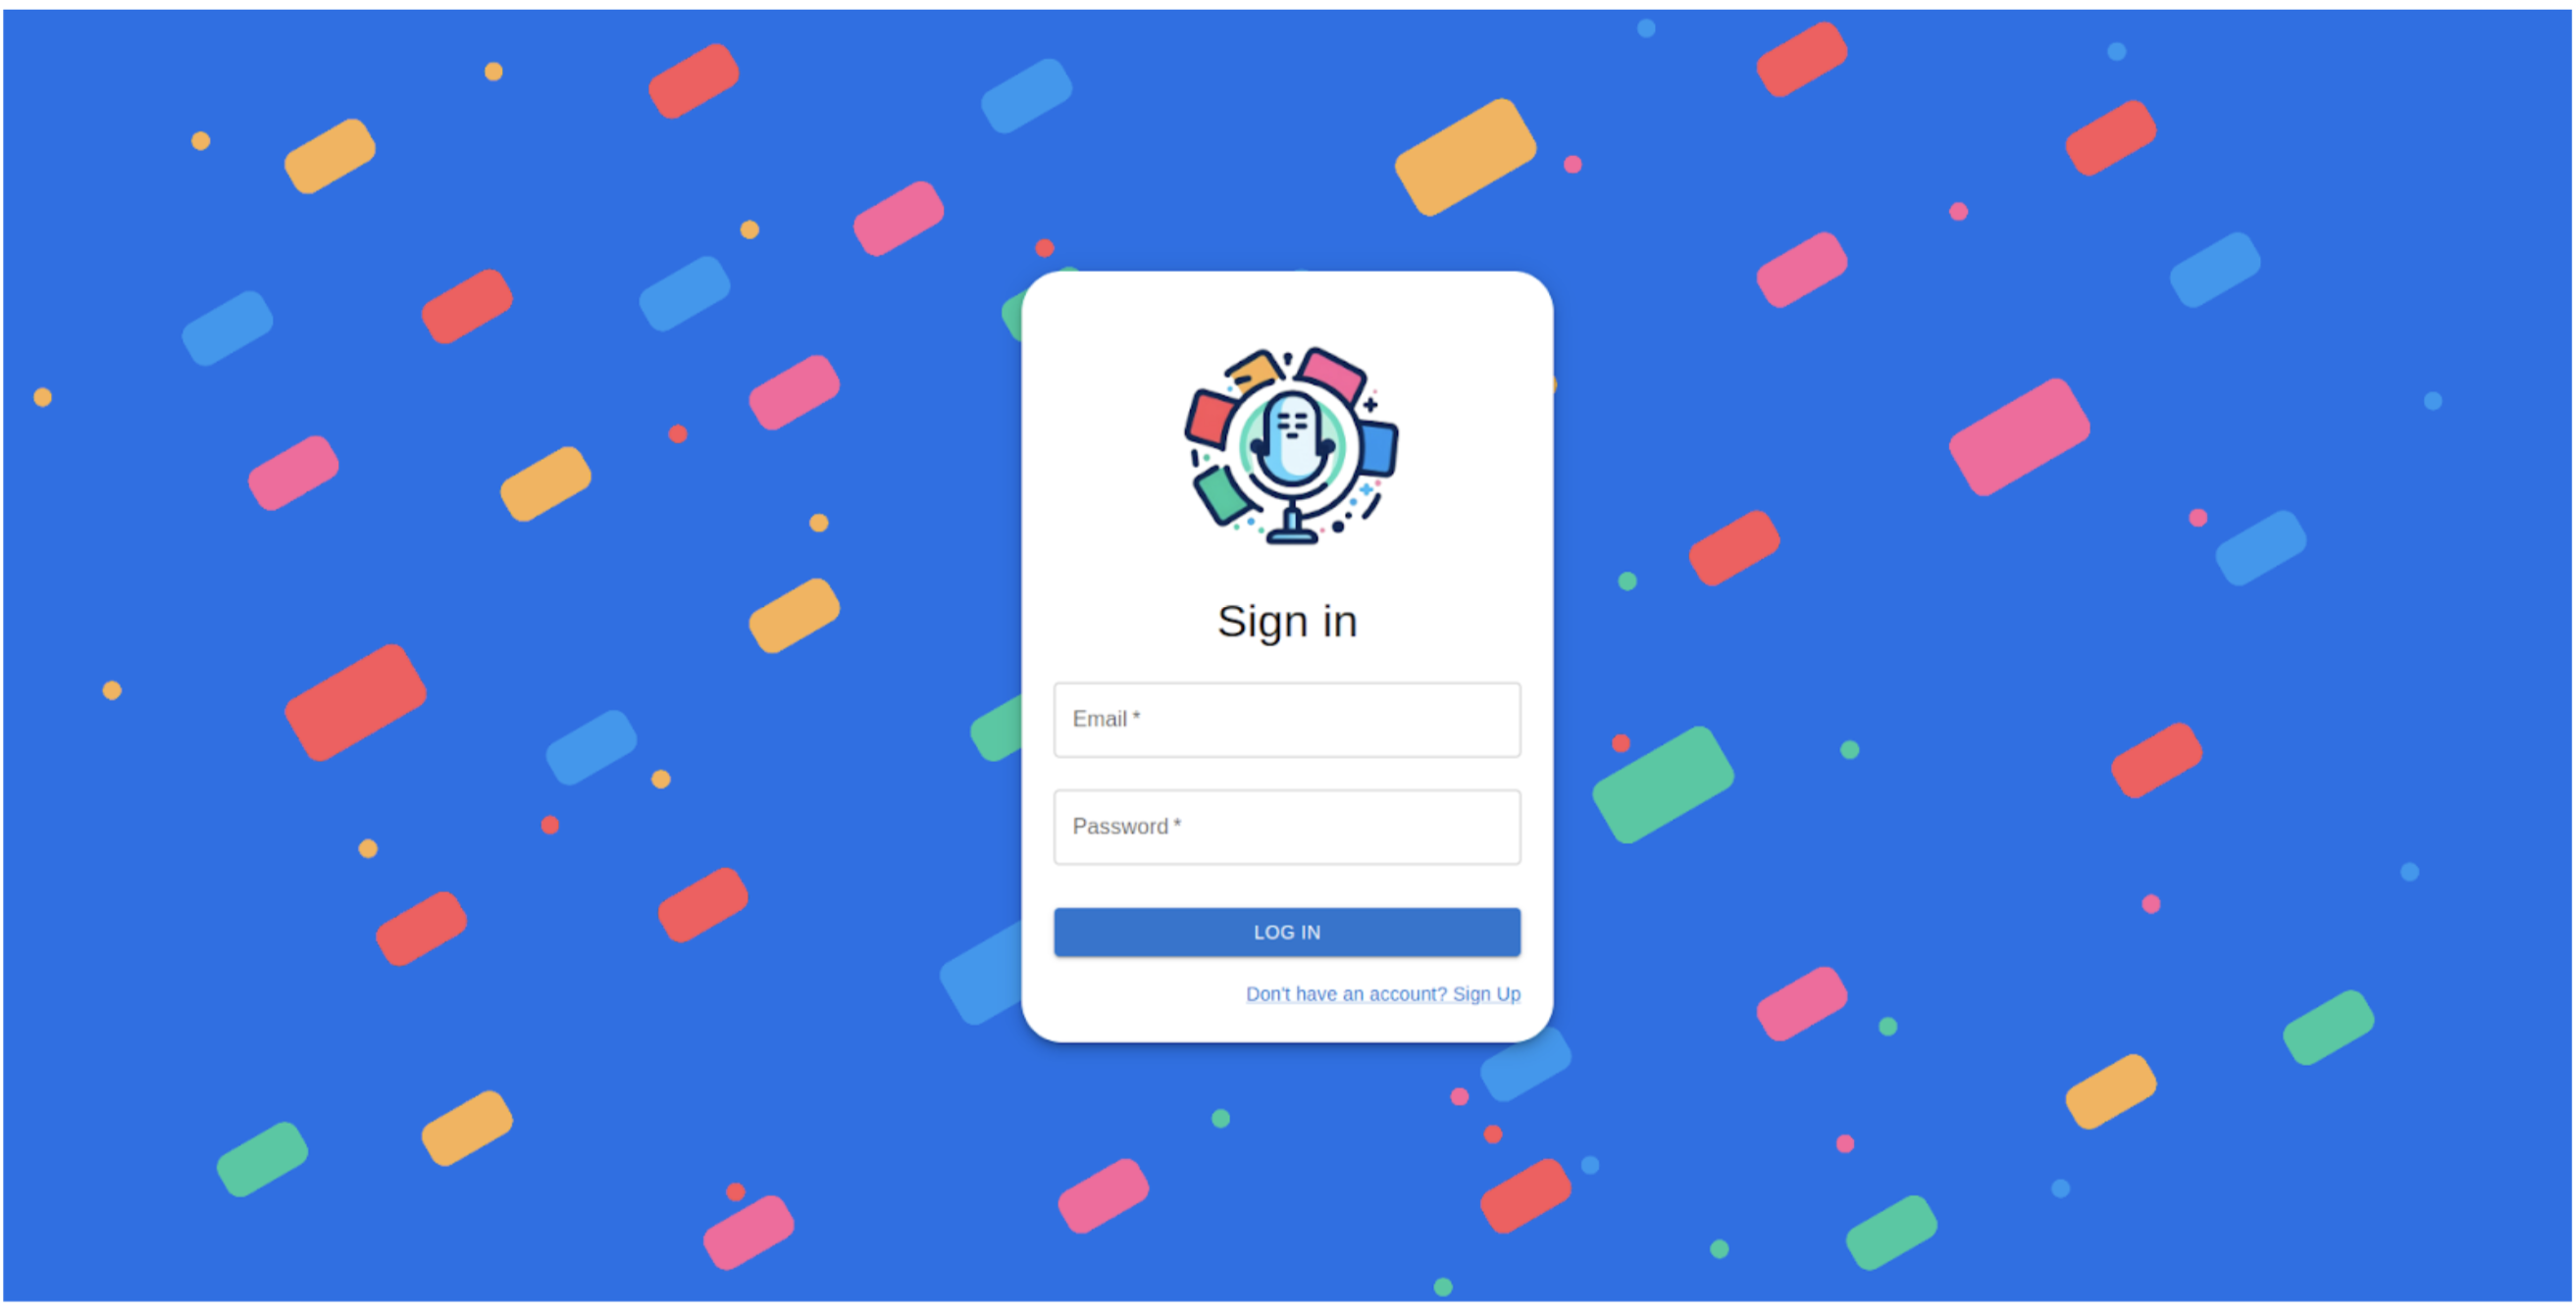
\includegraphics[width=0.9\textwidth]{chapters/chapter_10/images_web/web_login}
    \caption{Widok logowania.}
    \label{img:web_login}
\end{figure}


\begin{figure}[H]
    \centering
    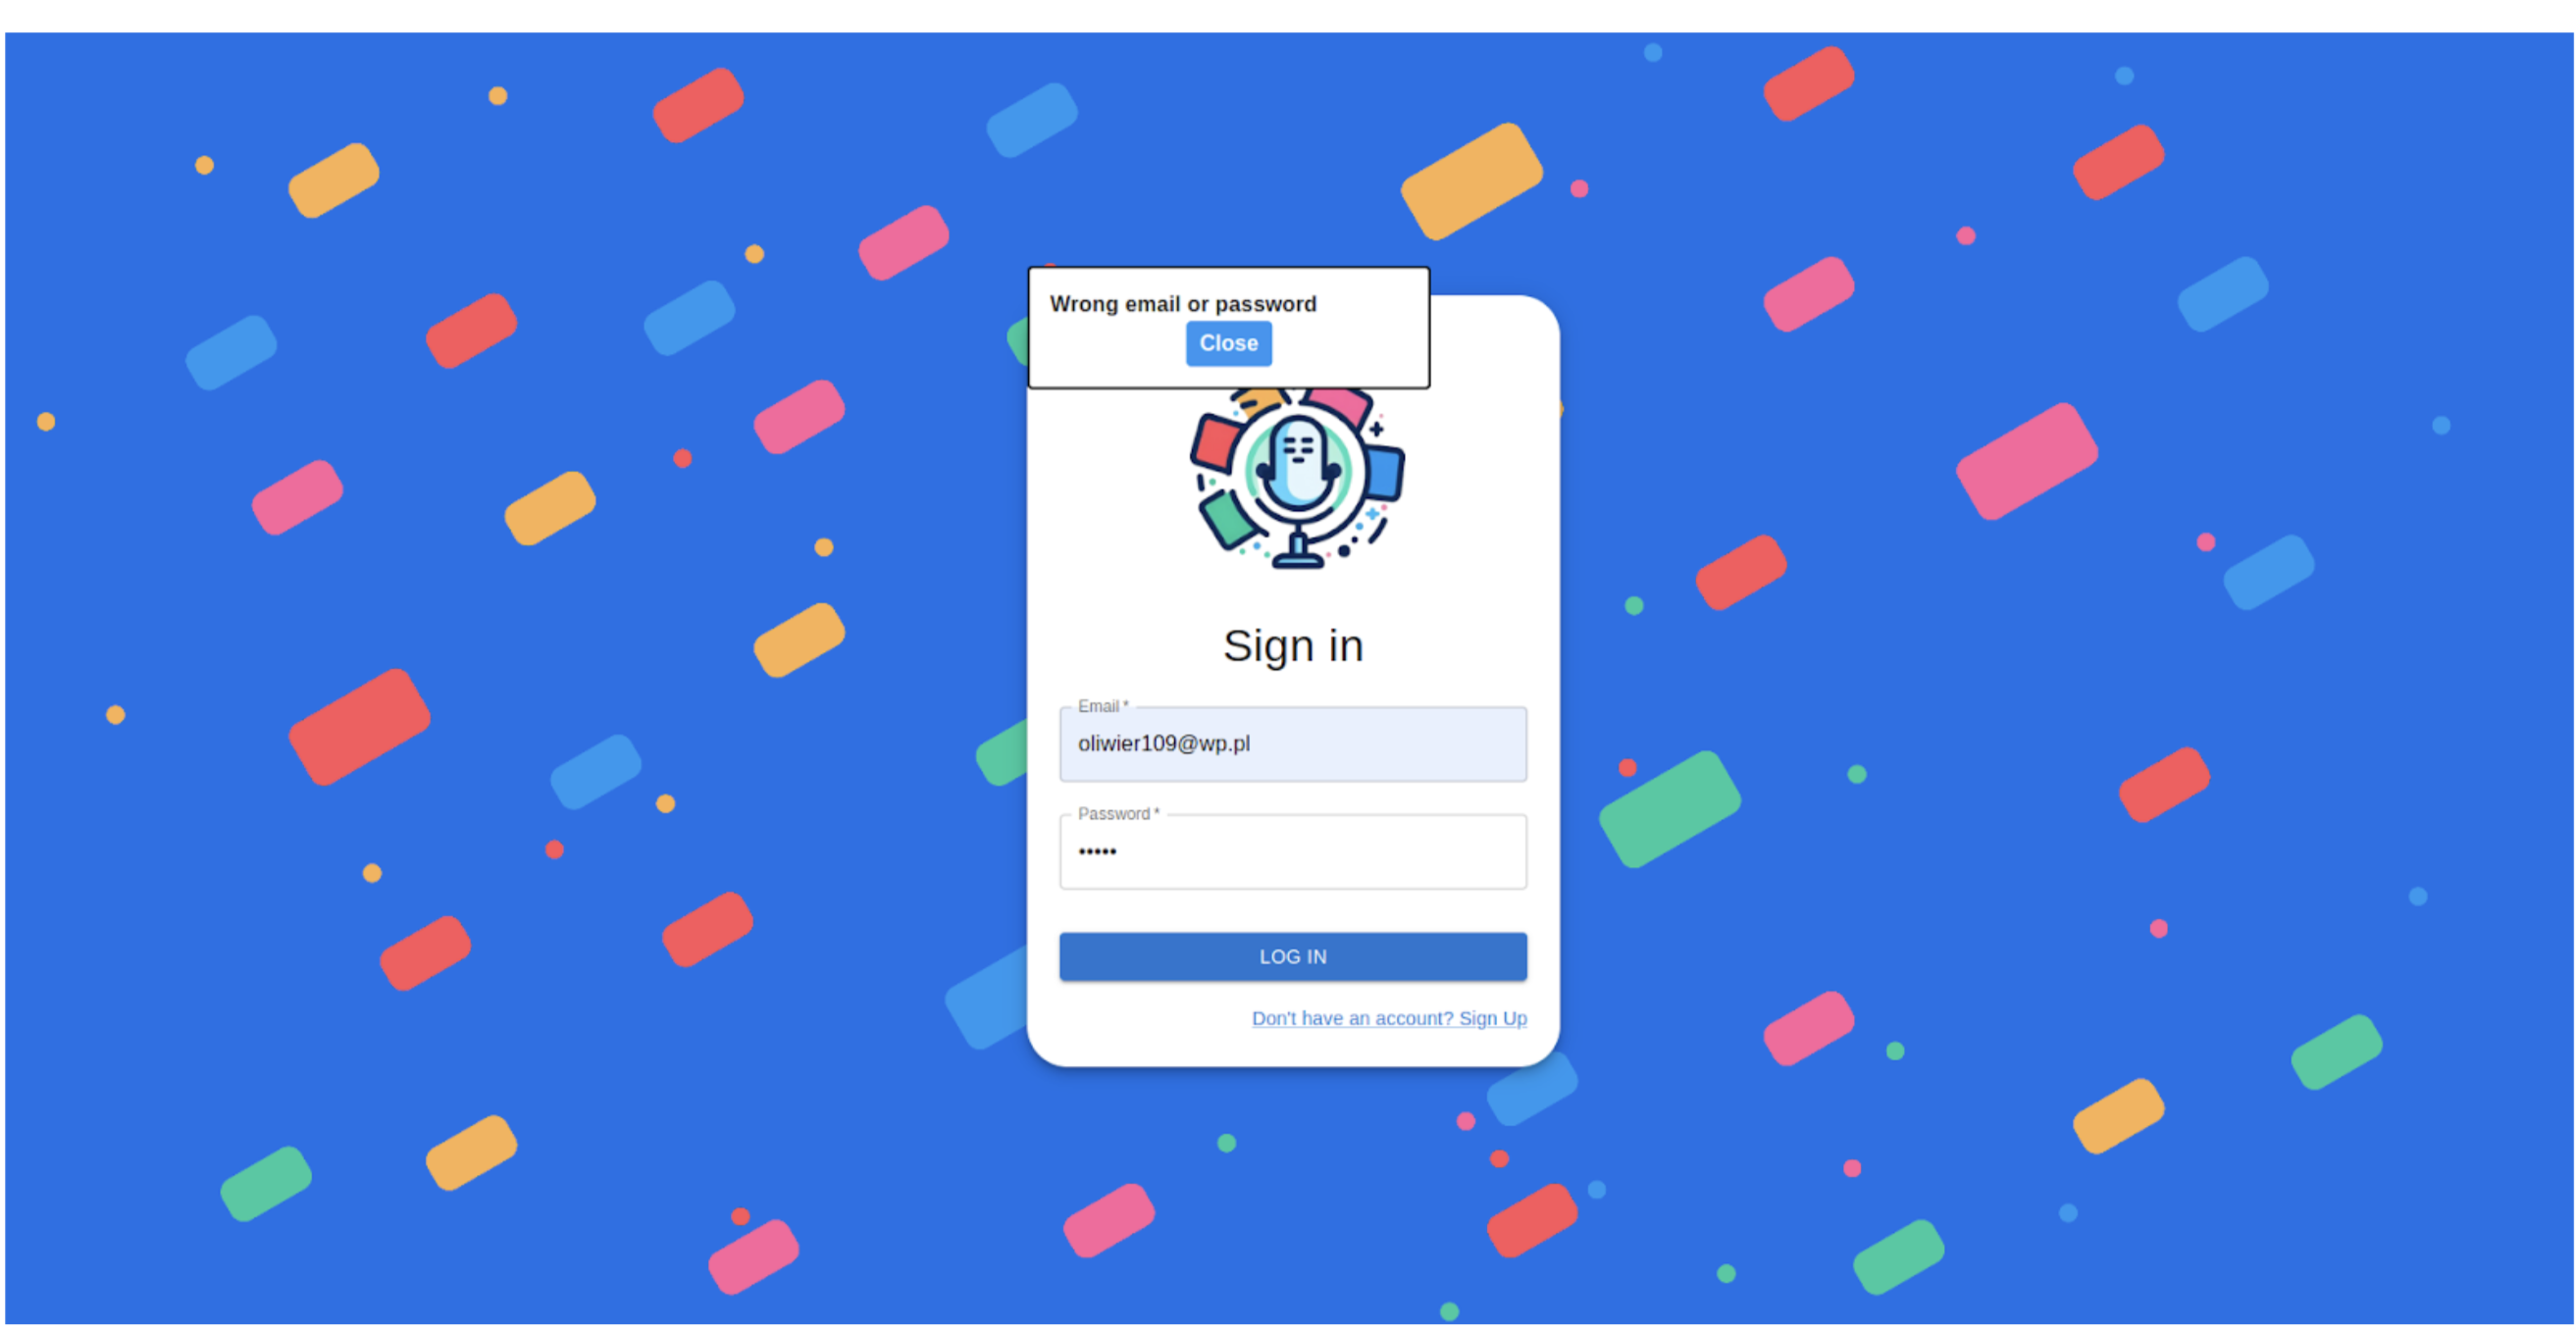
\includegraphics[width=0.9\textwidth]{chapters/chapter_10/images_web/web_login_2}
    \caption{Widok logowania po wpisaniu nieprawidłowych danych logowania.}
    \label{img:web_login_2}
\end{figure}


\subsection{Rejestracja}
Rejestracja pozwala na utworzenie konta potrzebnego do logowania.


\begin{figure}[H]
    \centering
    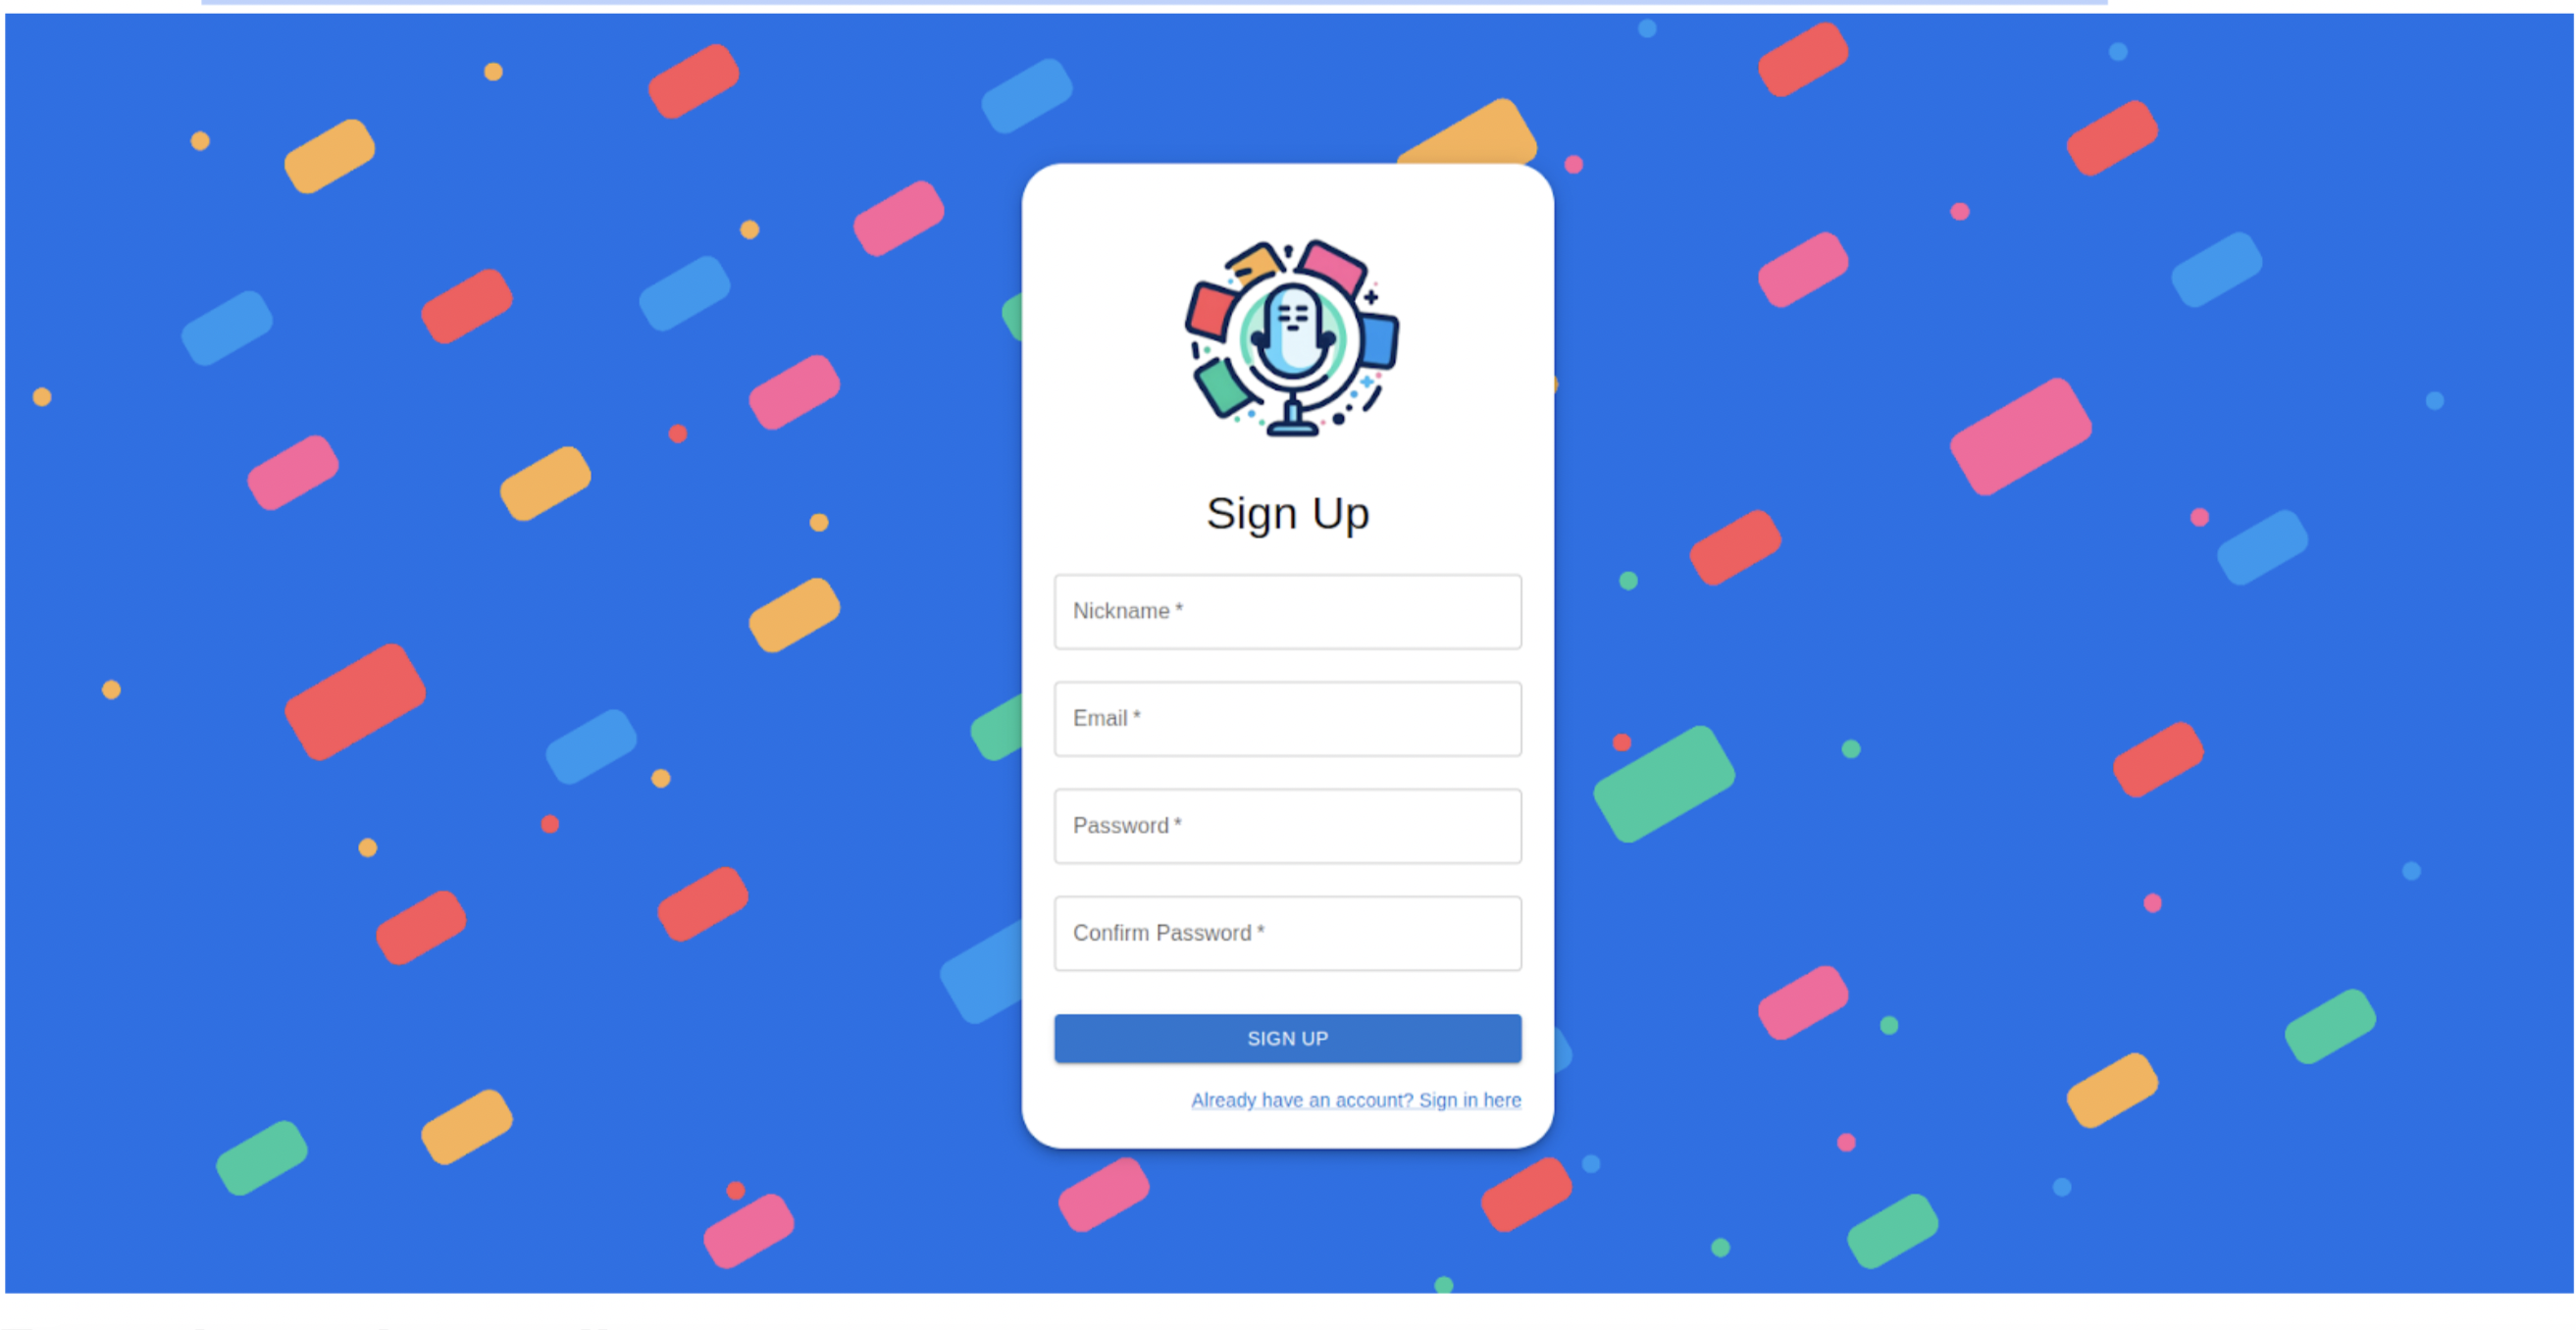
\includegraphics[width=0.9\textwidth]{chapters/chapter_10/images_web/web_register}
    \caption{Formularz rejestracji.}
    \label{img:web_register}
\end{figure}


\begin{figure}[H]
    \centering
    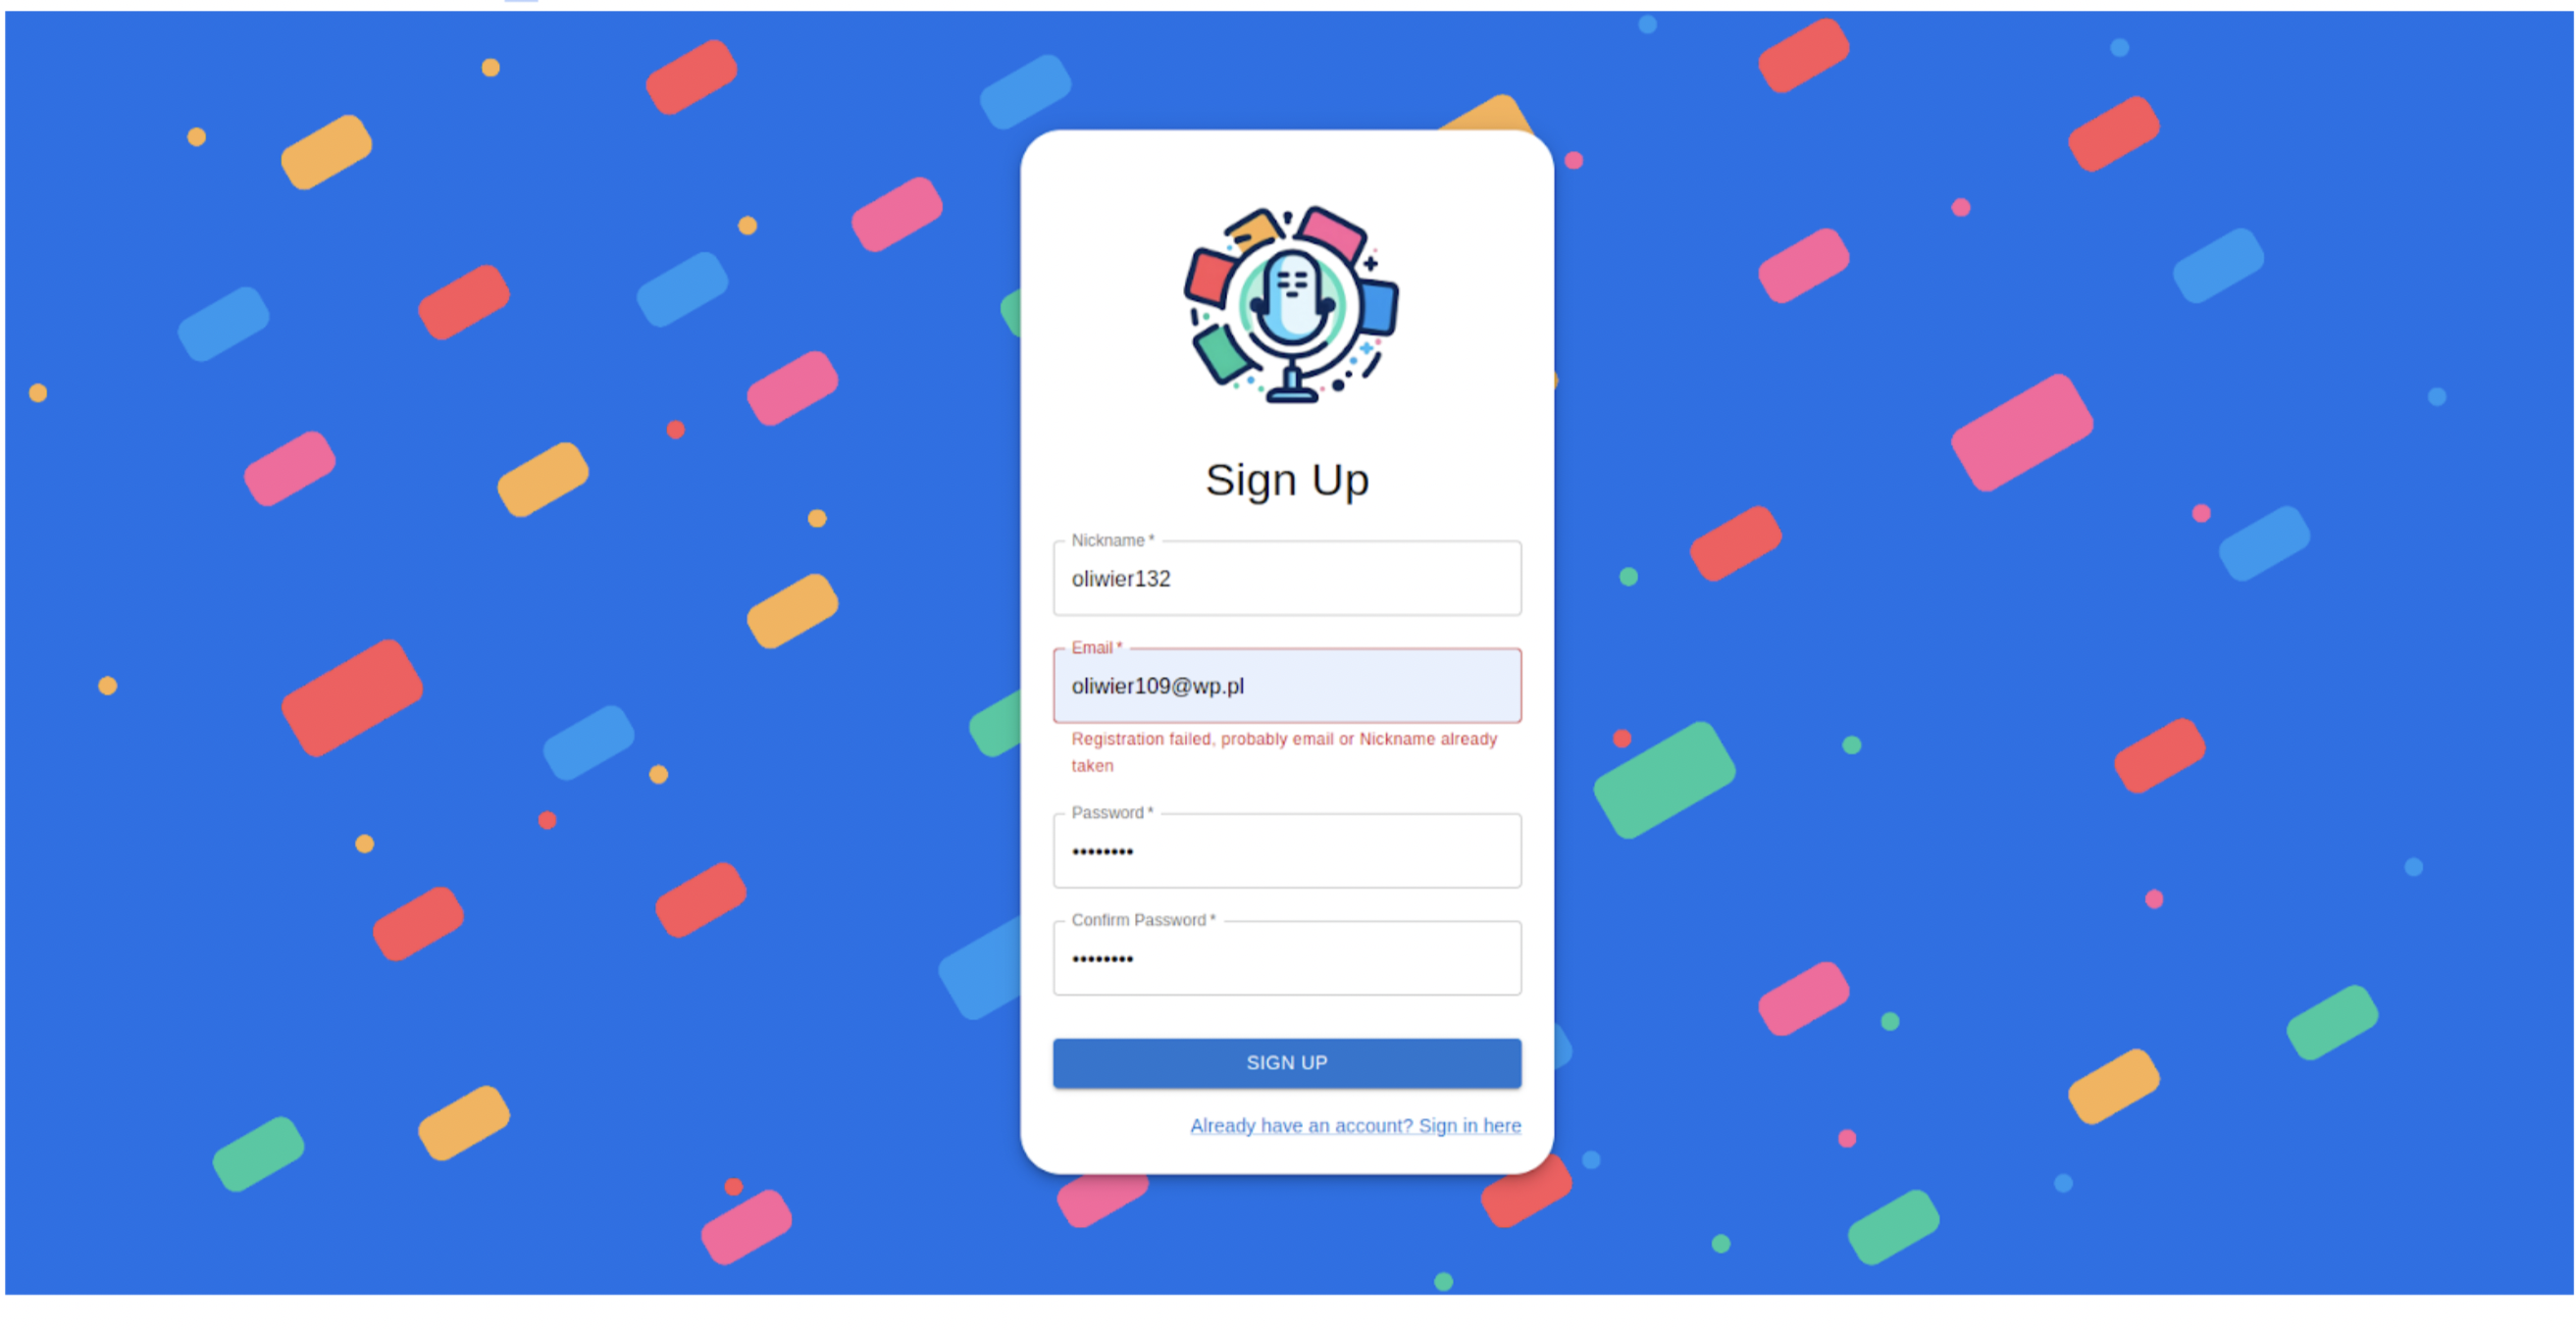
\includegraphics[width=0.9\textwidth]{chapters/chapter_10/images_web/web_register_2}
    \caption{Błąd po nieudanej rejestracji konta.}
    \label{img:web_register_2}
\end{figure}


\subsection{Strona domowa}
Po zalogowaniu użytkownik zostaje przekierowany do strony domowej. Na stronie domowej użytkownika możliwość wylogowania się lub może przejść do któregoś z podanych widoków:
\begin{itemize}
    \item "Create Decks";
    \item "My Decks";
    \item "Public Decks";
    \item "Profile";
    \item "Ranking".
\end{itemize}


\begin{figure}[H]
    \centering
    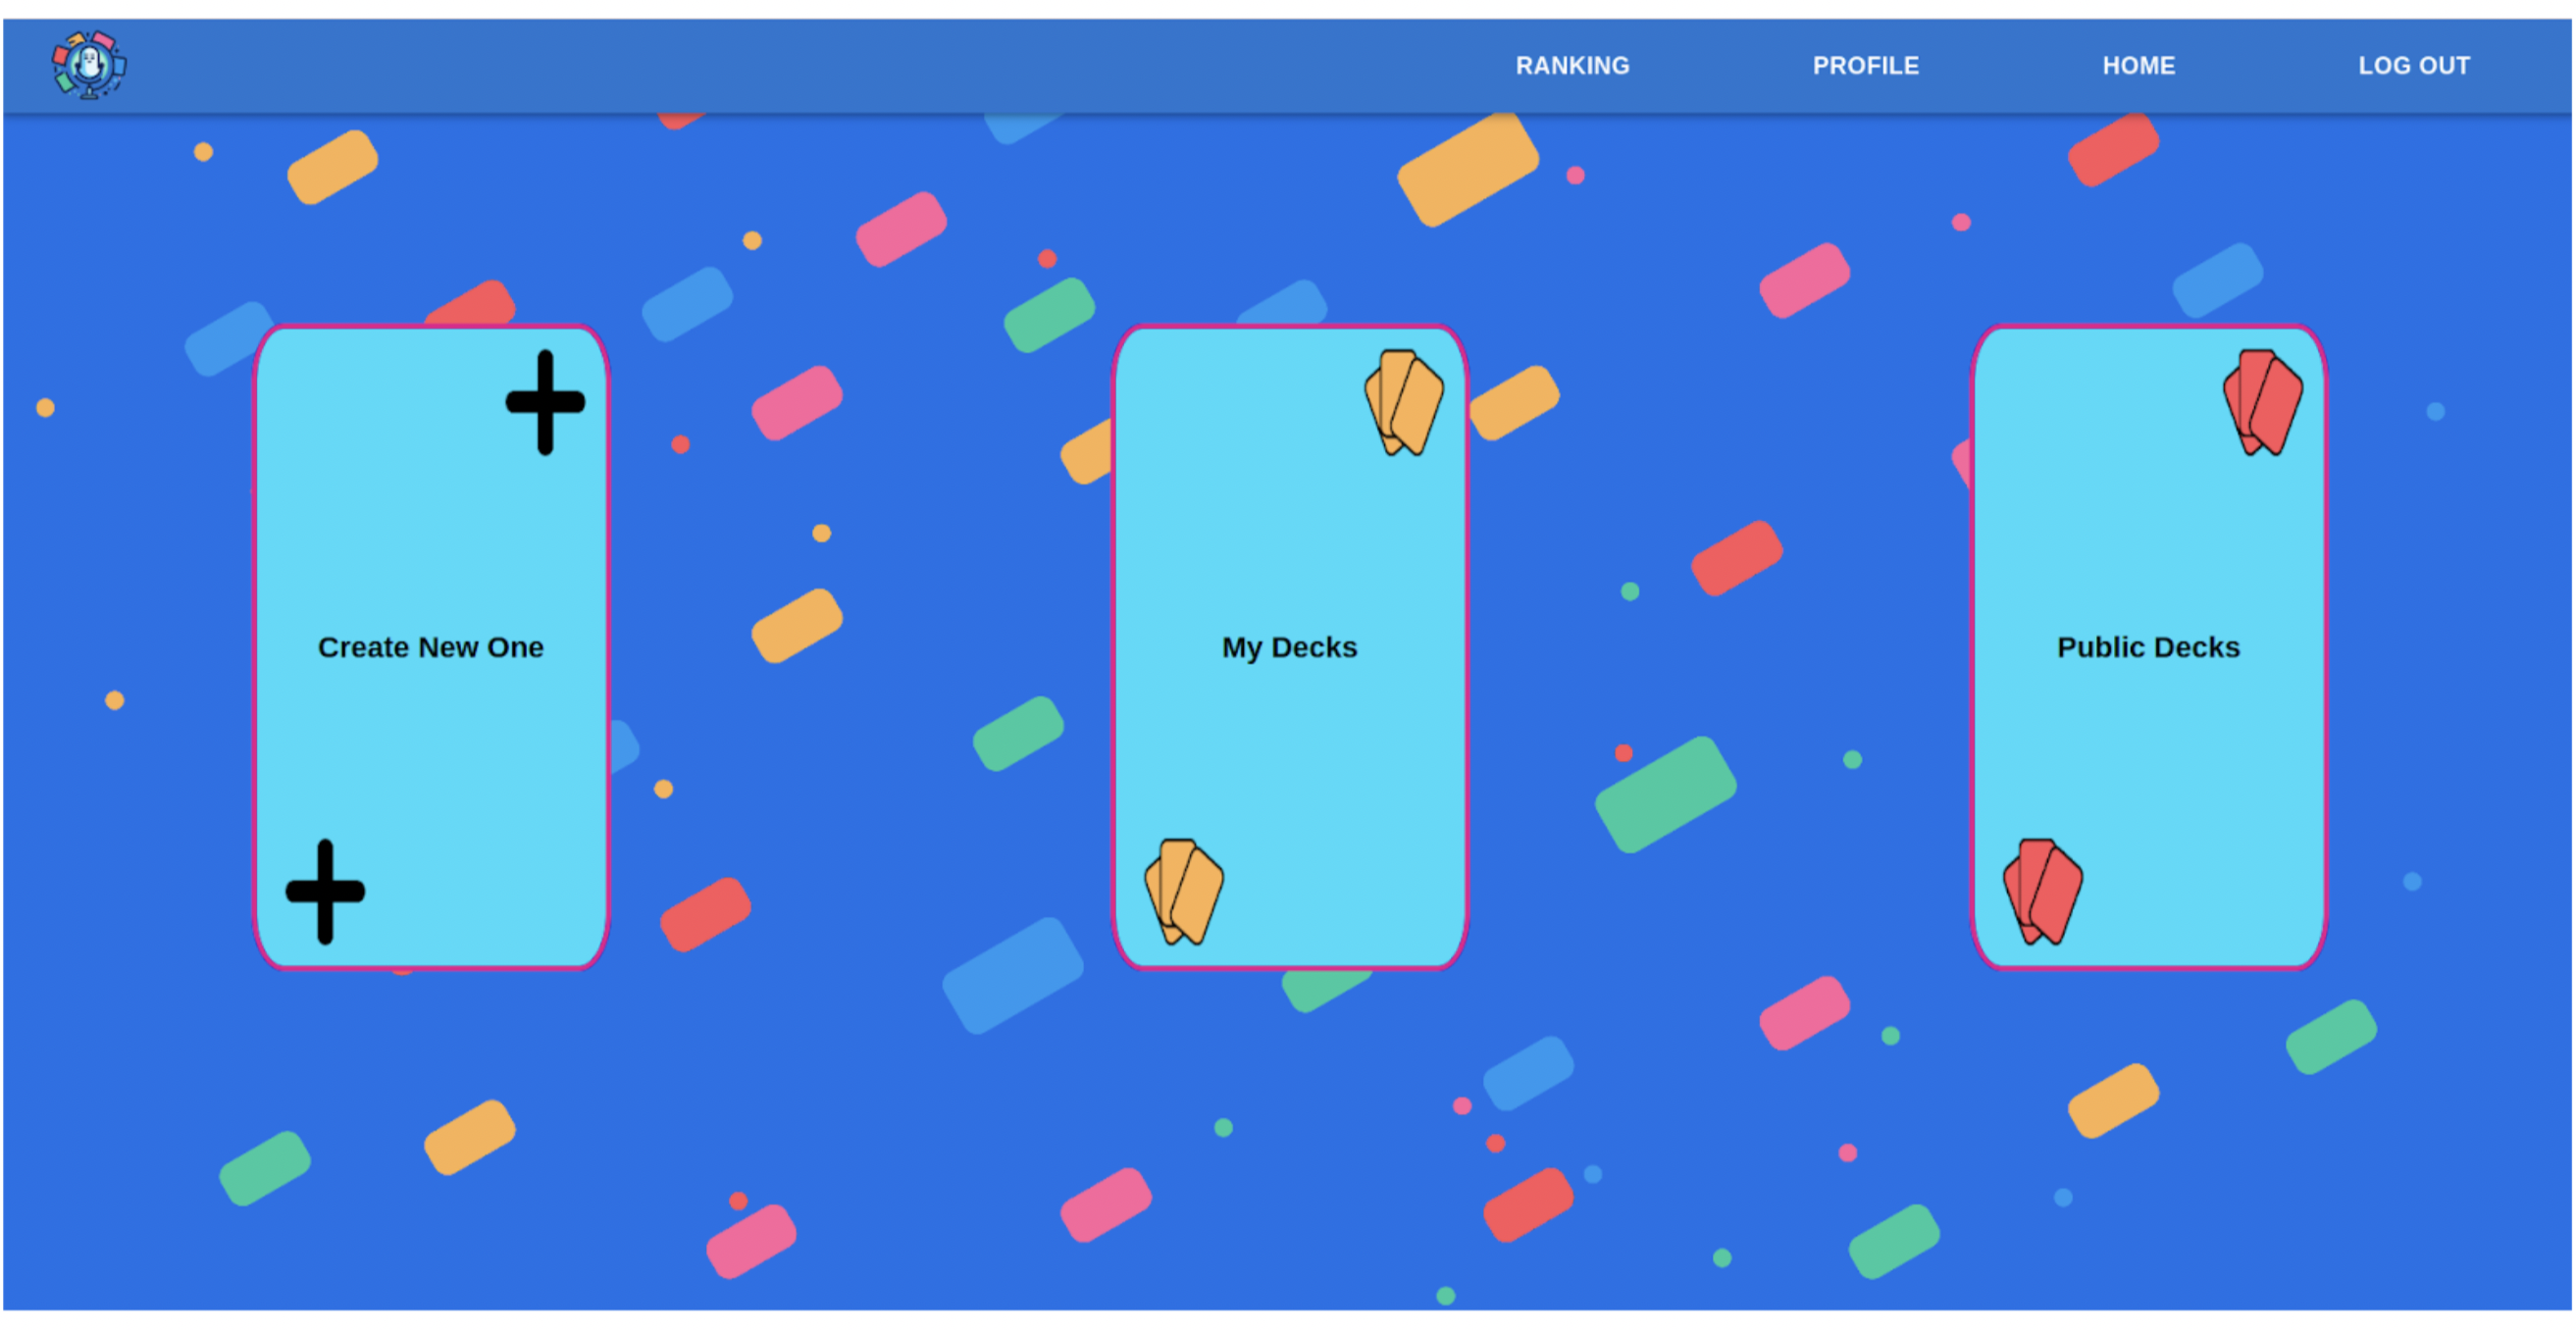
\includegraphics[width=0.9\textwidth]{chapters/chapter_10/images_web/web_home}
    \caption{Strona domowa.}
    \label{img:web_home}
\end{figure}


\subsection{Profil użytkownika}
Strona przedstawia profil użytkownika. Użytkownik ma możliwość zmiany swoich danych, usunięcia konta oraz przejścia do widoku ze swoimi statystykami.


\begin{figure}[H]
    \centering
    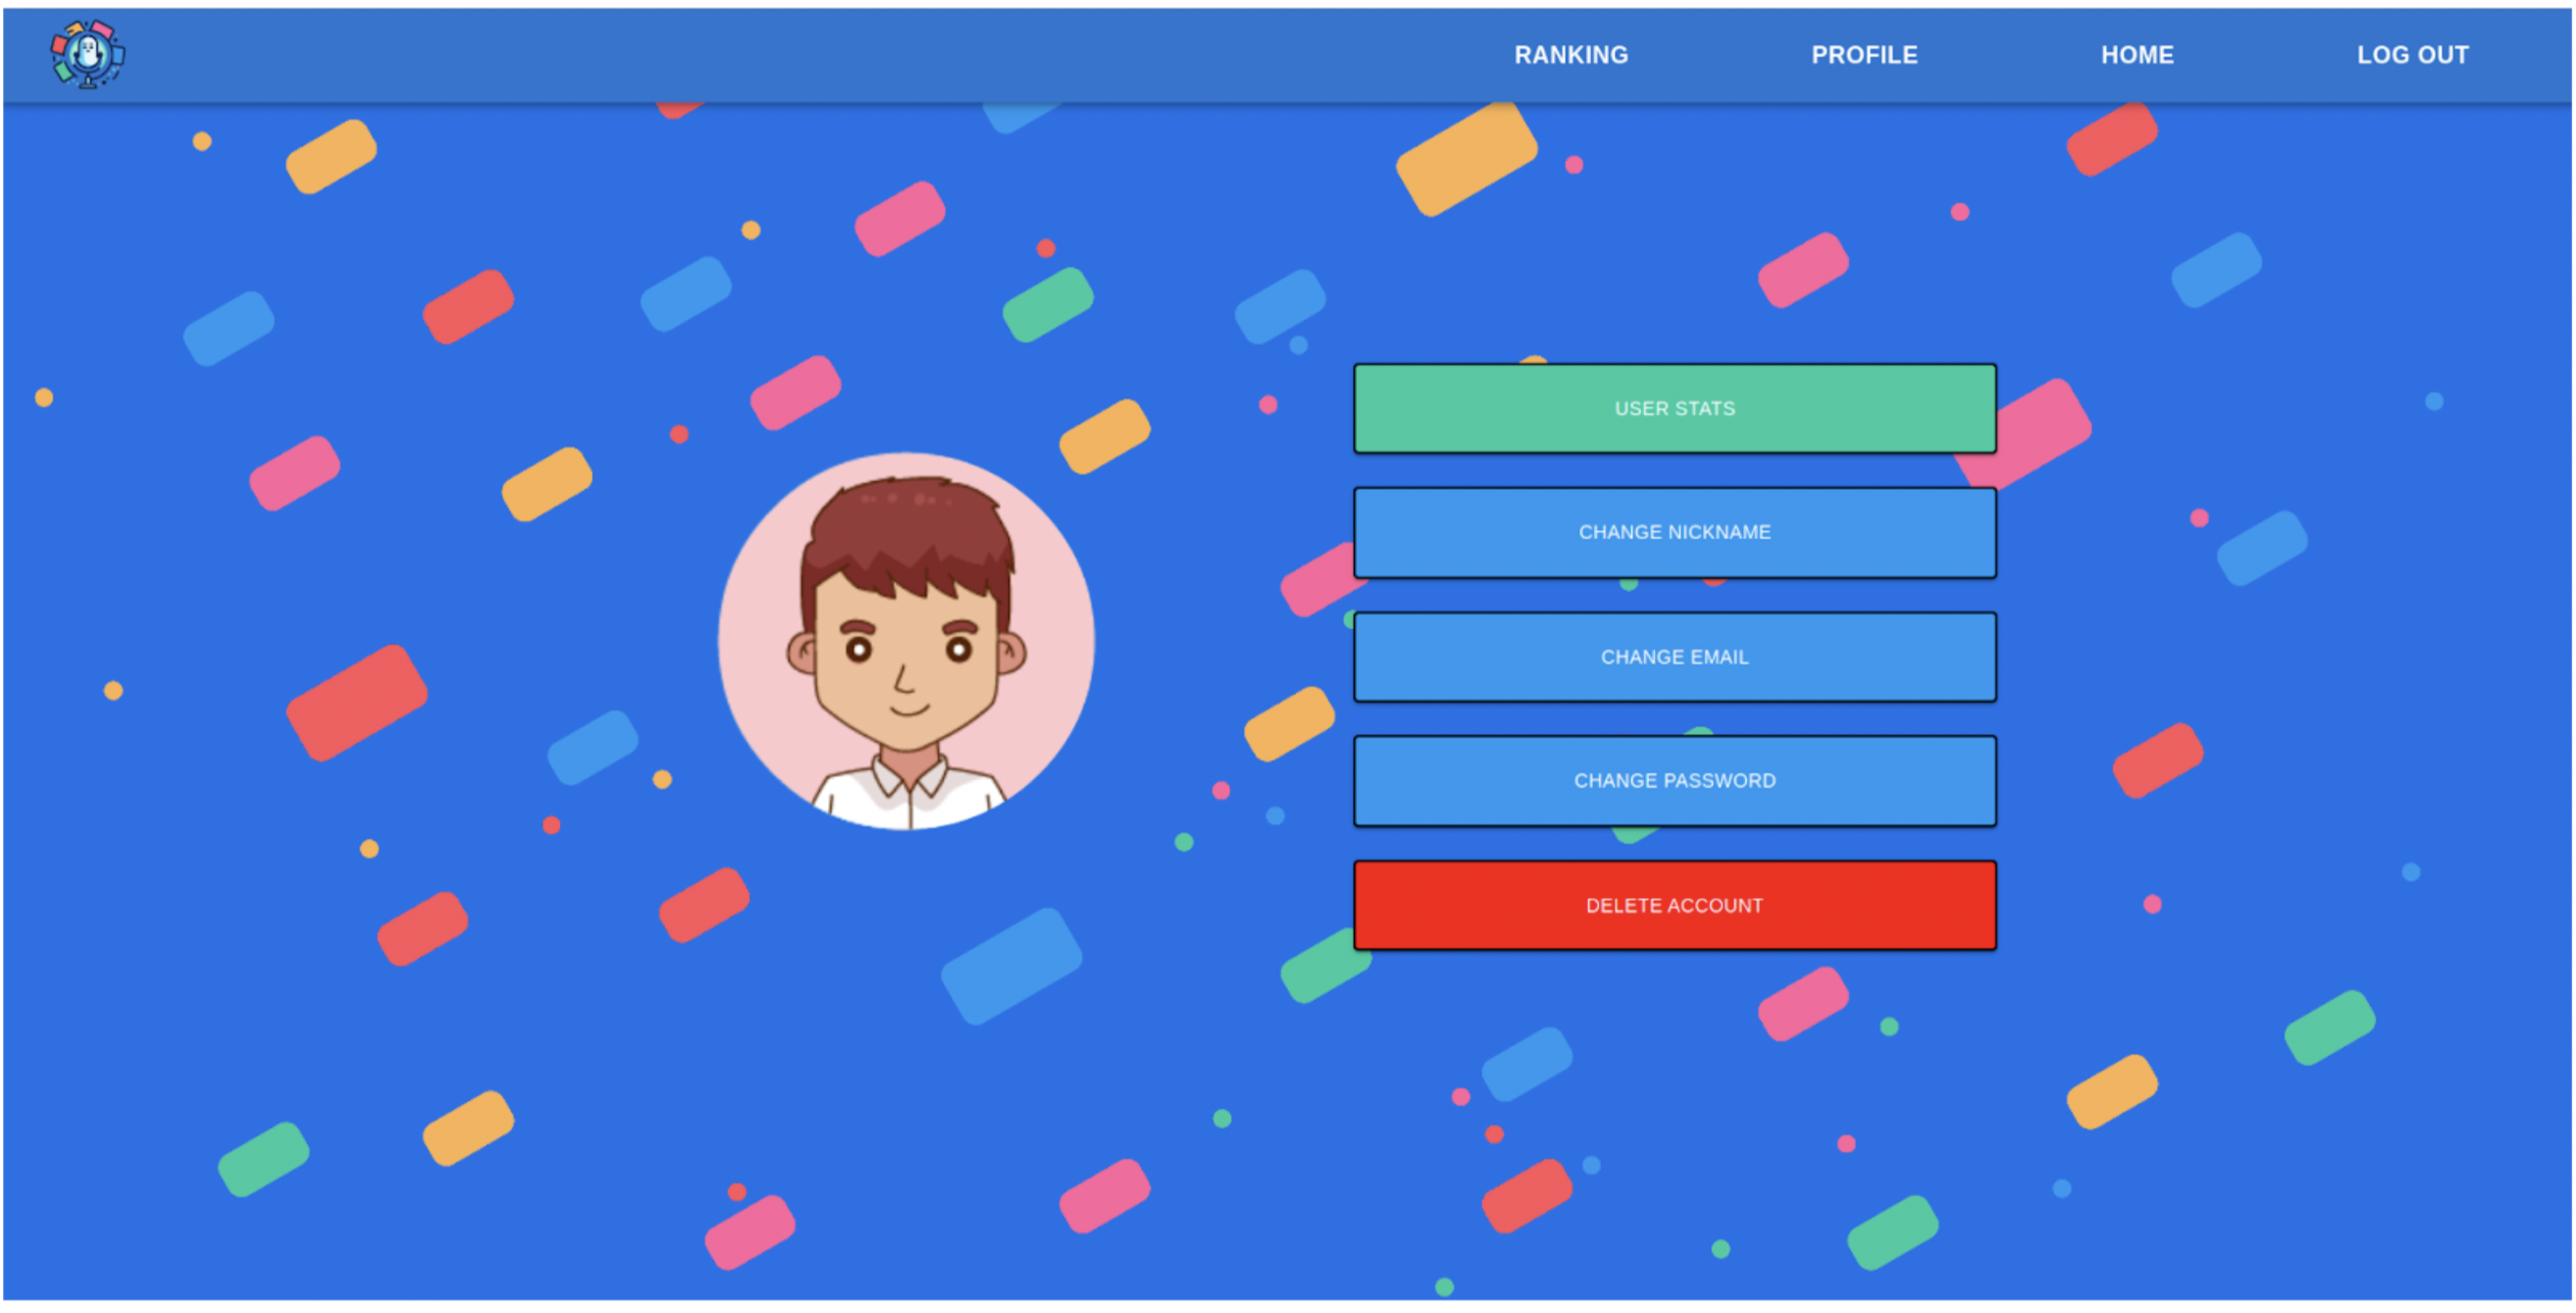
\includegraphics[width=0.9\textwidth]{chapters/chapter_10/images_web/web_profile}
    \caption{Profil użytkownika.}
    \label{img:web_profile}
\end{figure}


\begin{figure}[H]
    \centering
    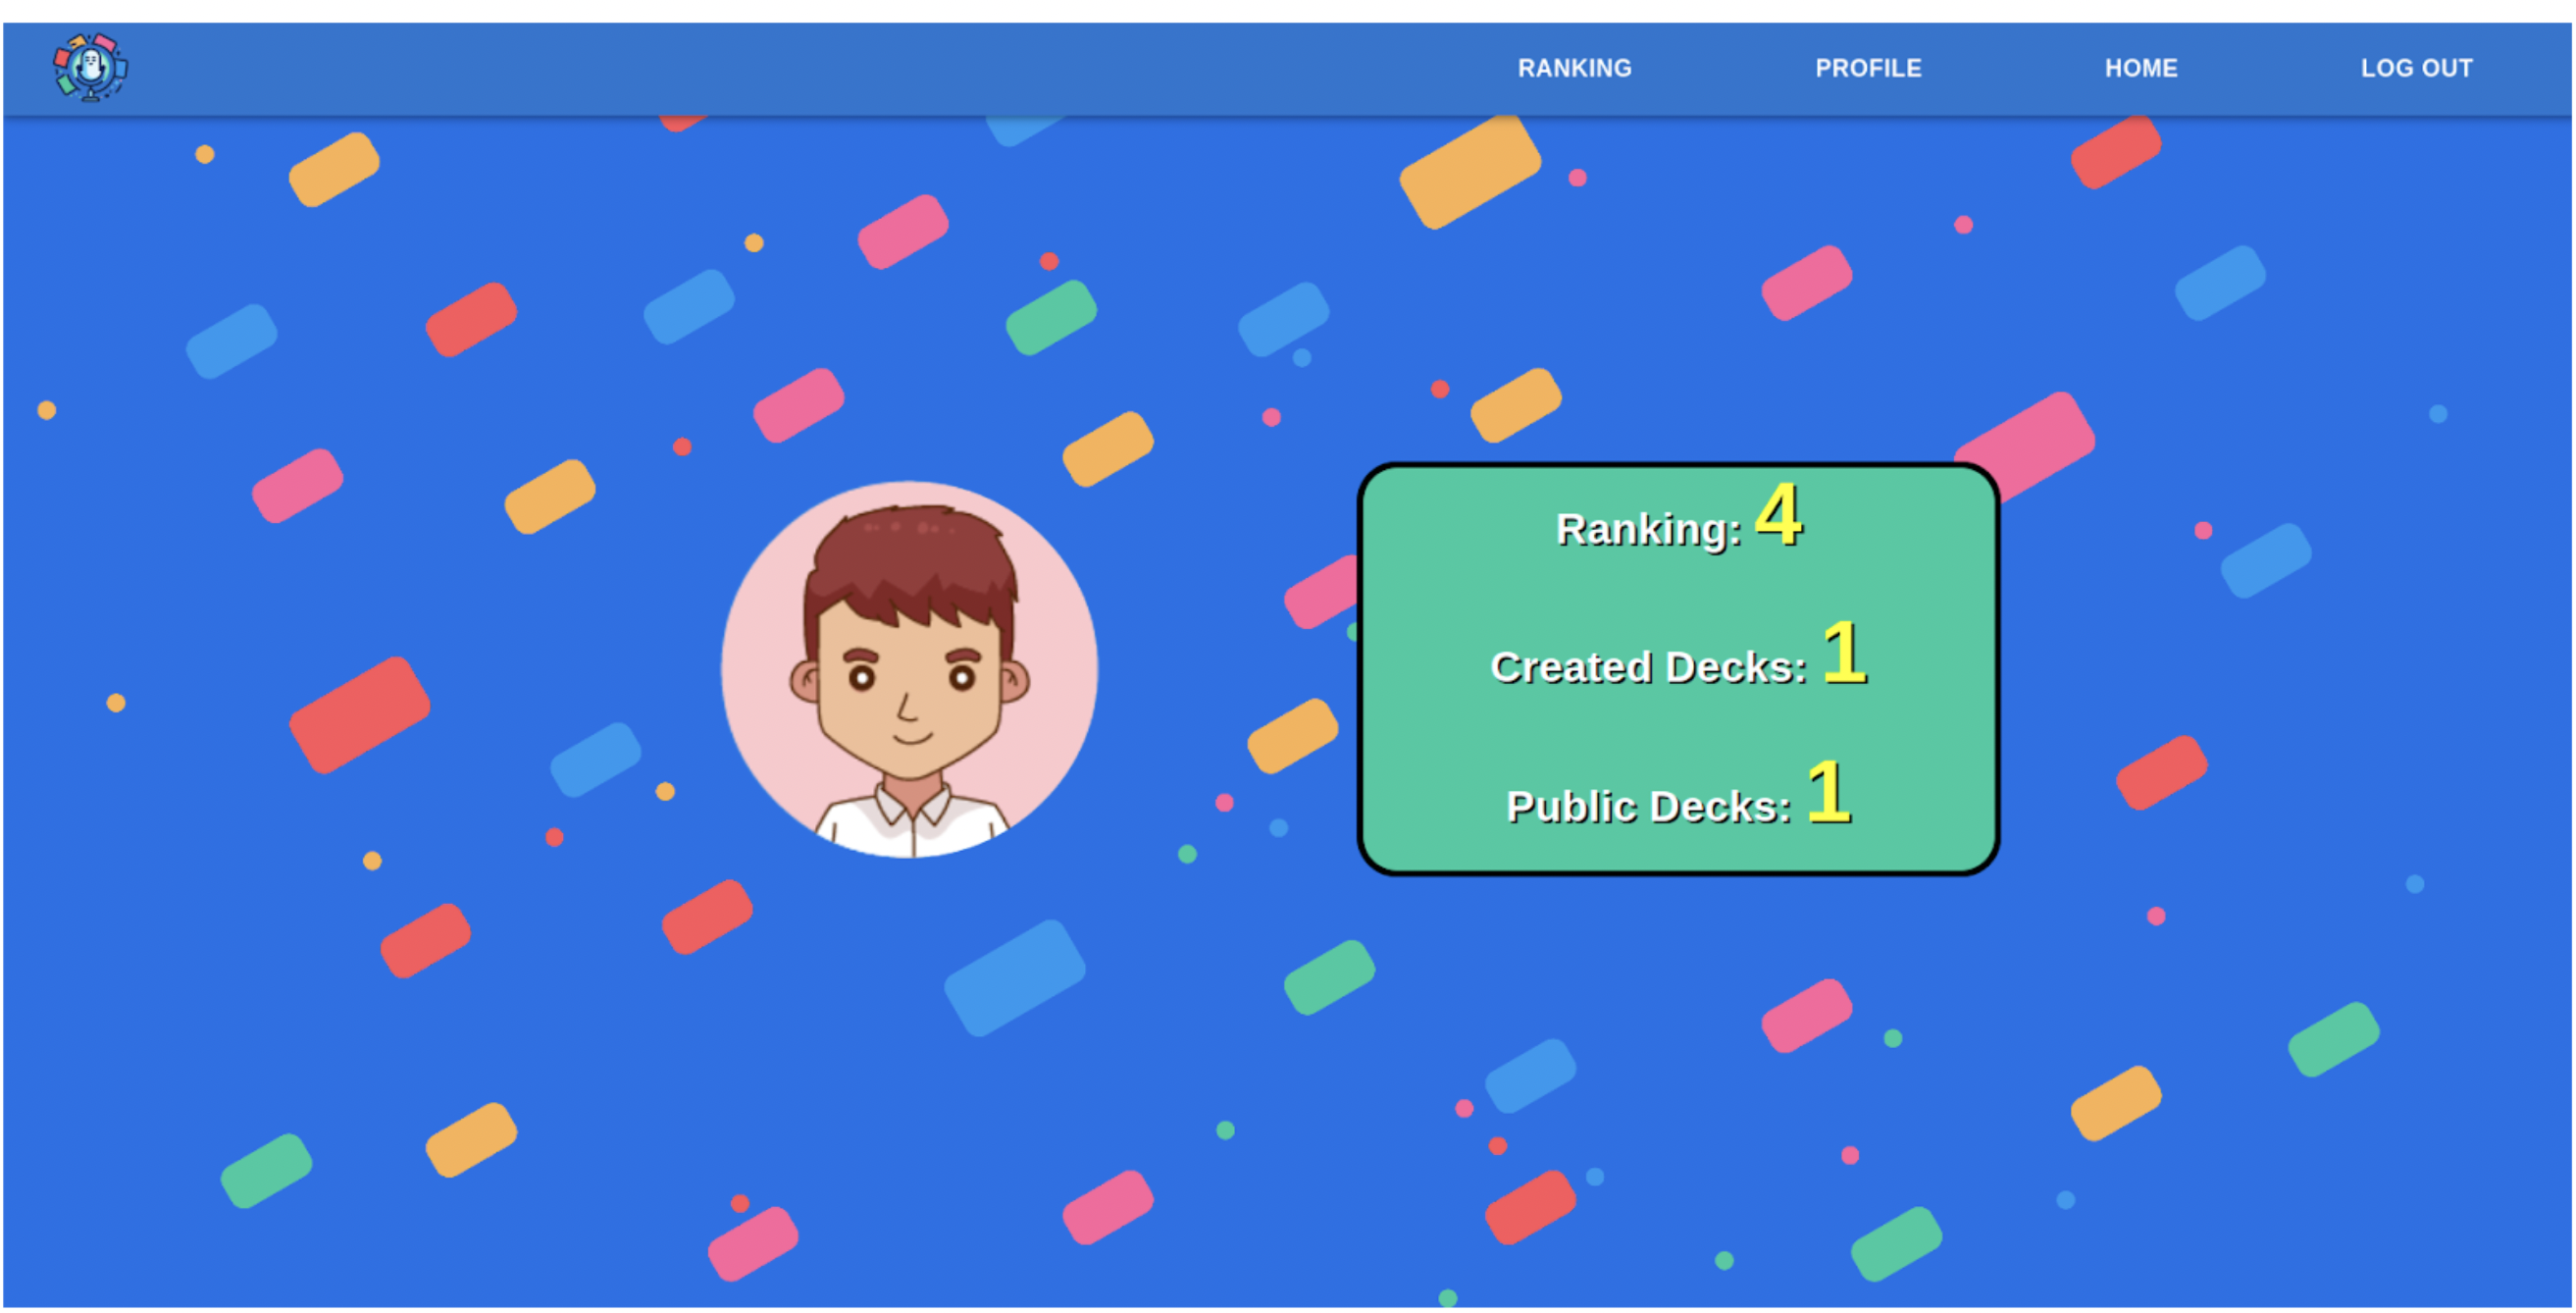
\includegraphics[width=0.9\textwidth]{chapters/chapter_10/images_web/web_stats}
    \caption{Statystyki użytkownika.}
    \label{img:web_stats}
\end{figure}


\subsection{"Create deck"}
Strona umożliwia tworzenie talii fiszek. Przycisk "Generate" pozwala na wygenerowanie treści fiszki używając ChatGPT. W celu utworzenia talii fiszek, użytkownik musi wypełnić nazwę talii, kategorię i mieć przynajmniej jedna wypłenione pole dla fiszki. Przycisk "Add card" dodaje następne pola do utworzenia fiszki. Użytkownik po wypełnieniu formularza musi kliknąć "Create deck" w celu utworzenia talii.


\begin{figure}[H]
    \centering
    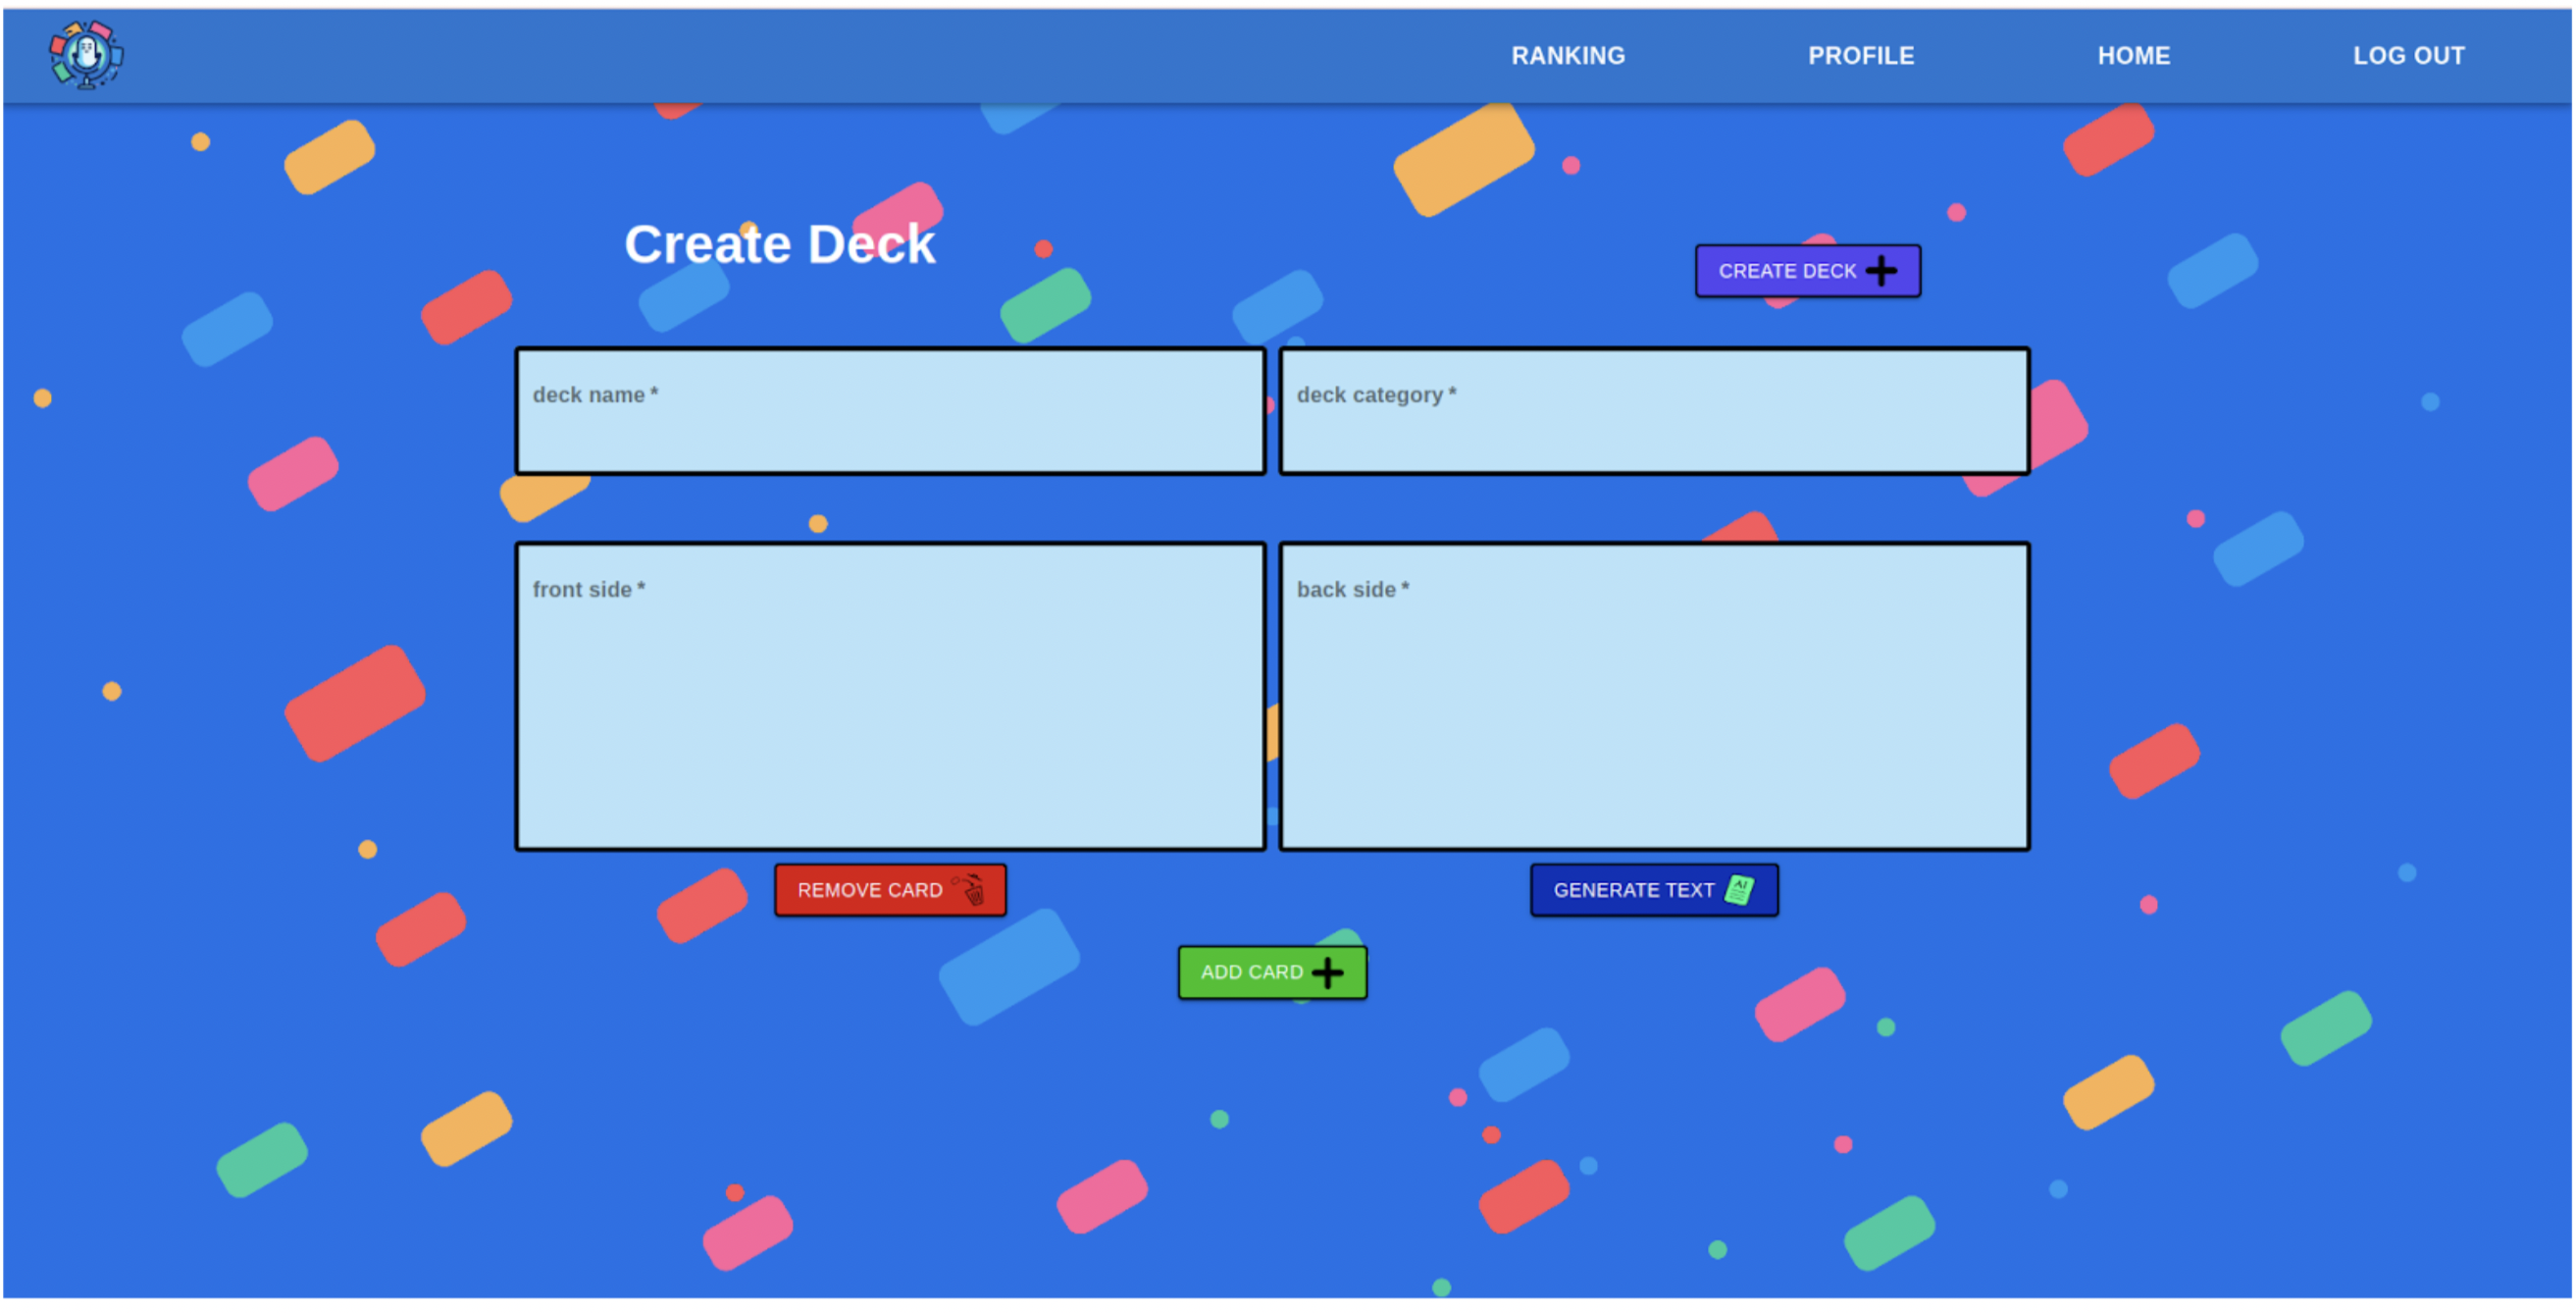
\includegraphics[width=0.9\textwidth]{chapters/chapter_10/images_web/web_create_deck}
    \caption{Widok tworzenia talii.}
    \label{img:web_create_deck}
\end{figure}


Użytkownik może wypełnić przednią stronę fiszki, następnie kliknięcie przycisku "Generate" pozwoli na wygenerowanie przez ChatGPT tekstu na podstawie zawartości przedniej strony fiszki. Po wygenerowaniu treść pojawi się w okienku i użytkownik ma możliwość zaakceptowania treści lub jej odrzucenia. W przypadku zaakceptowania tylna strona fiszki zostanie wypełniona wygenerowaną treścią.


\begin{figure}[H]
    \centering
    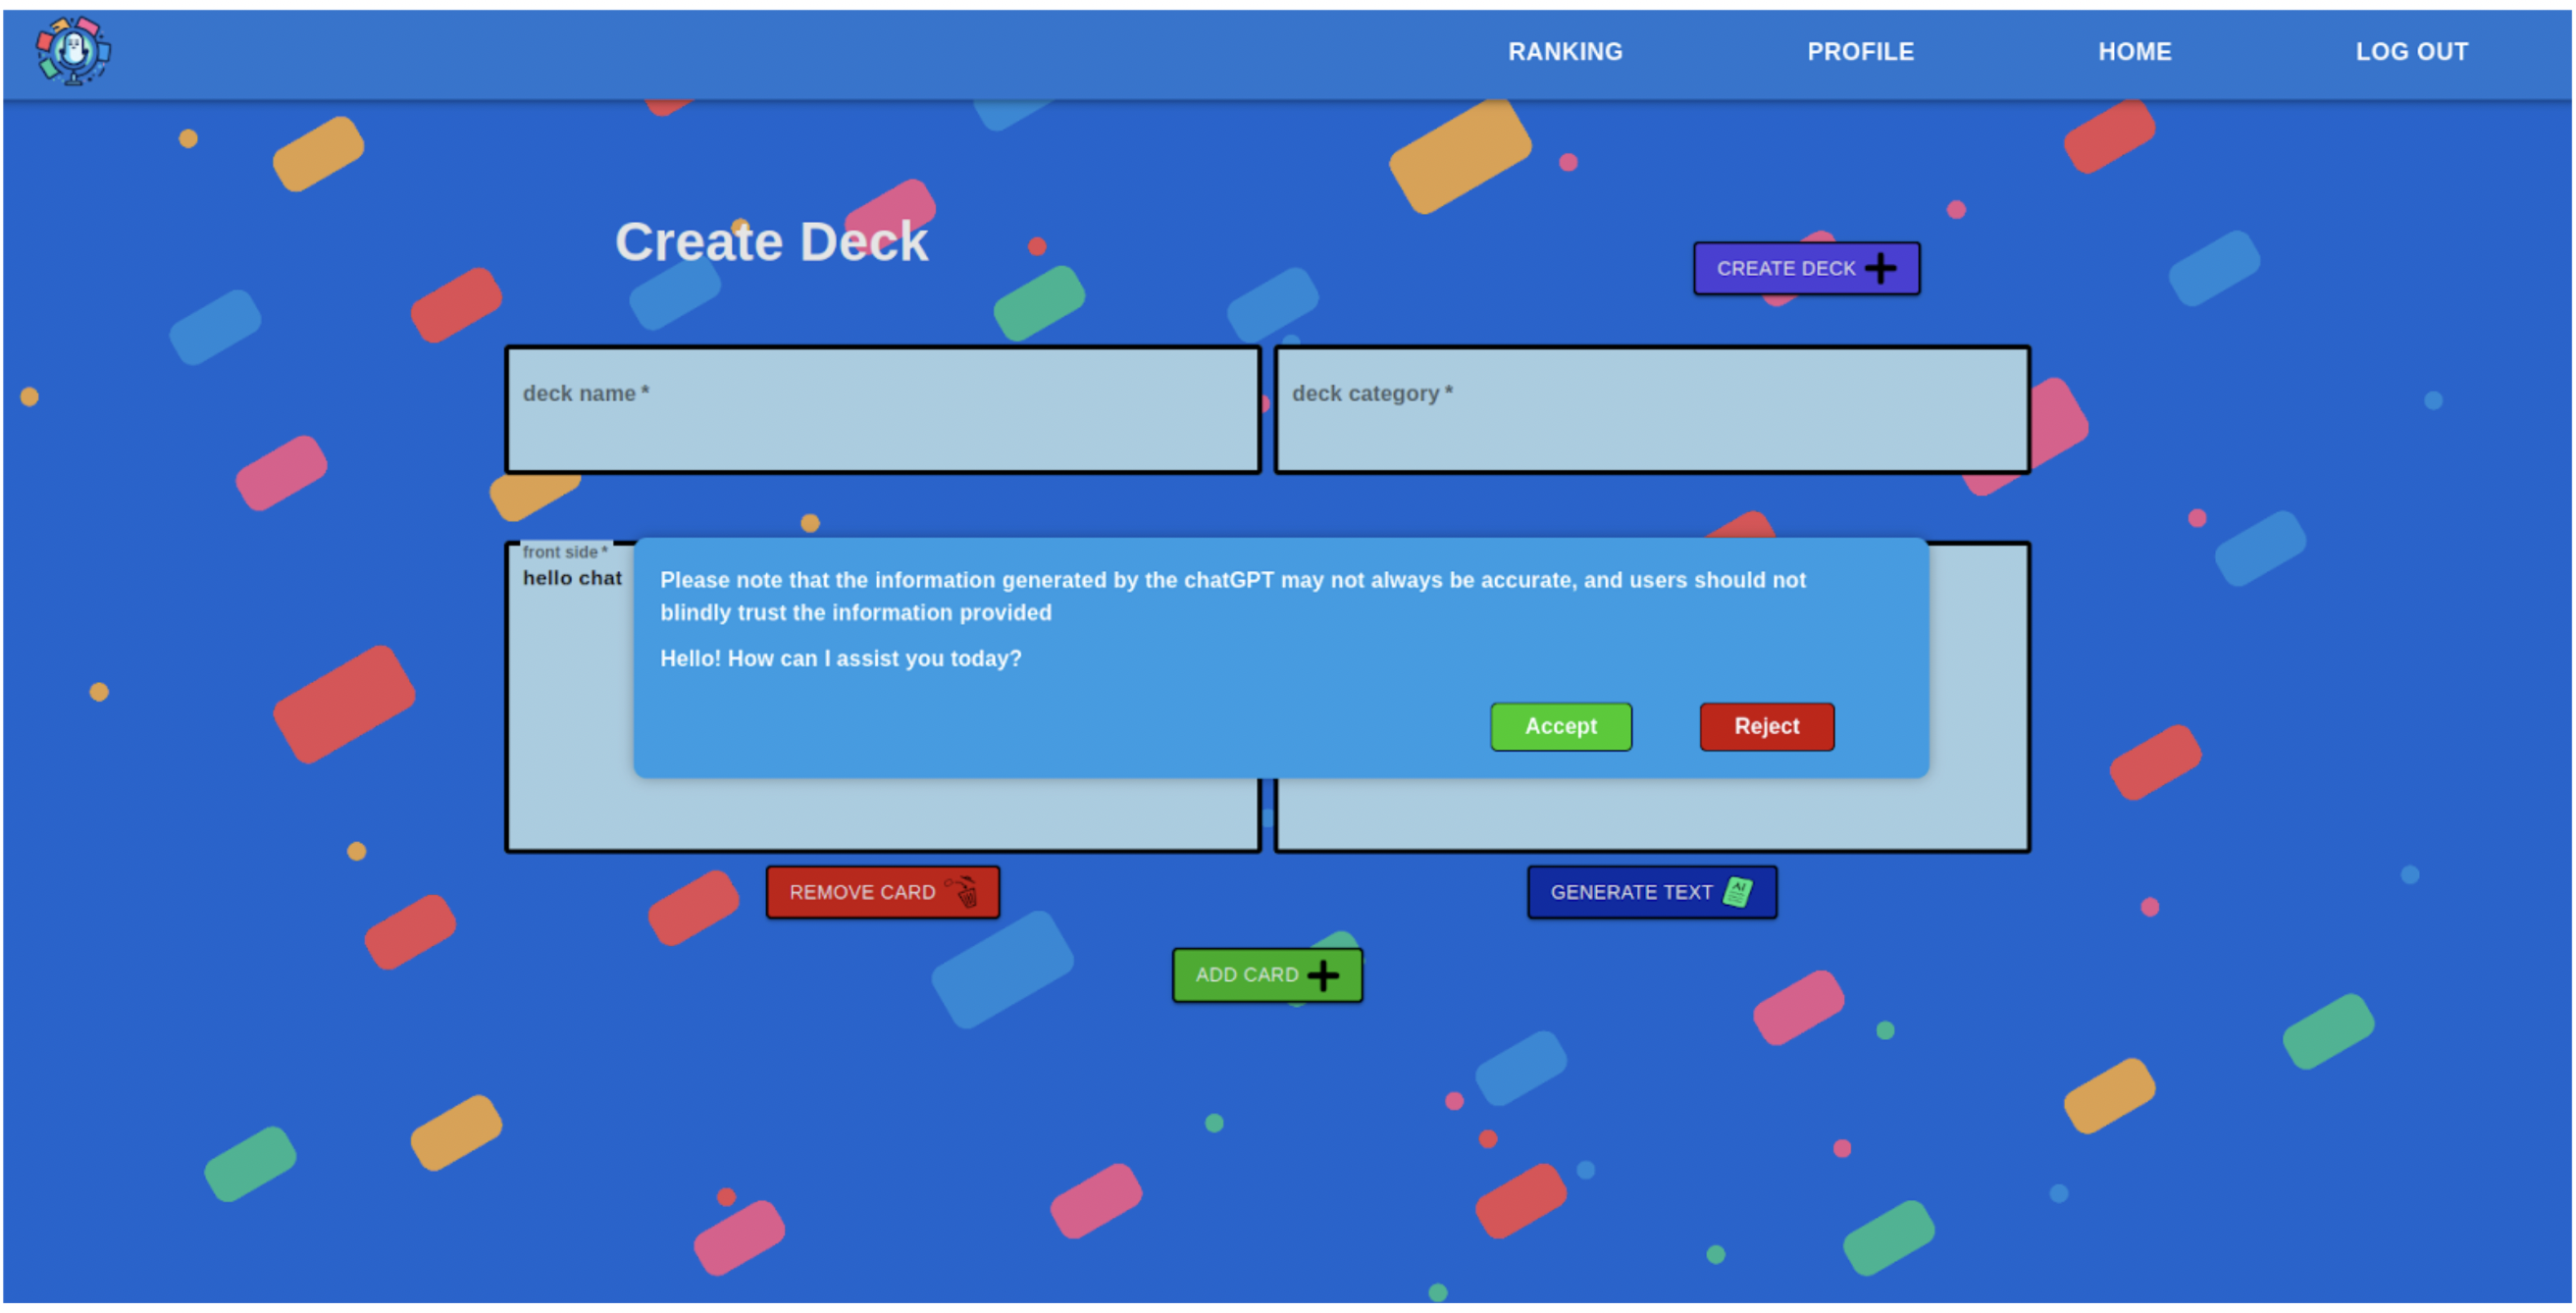
\includegraphics[width=0.9\textwidth]{chapters/chapter_10/images_web/web_chat}
    \caption{Generowanie treści przez ChatGPT.}
    \label{img:web_chat}
\end{figure}


\subsection{"My Decks"}
W "My decks" trzymane są wszystkie talie utworzone przez użytkownika. Filter pozwala na wyszukiwanie talii jednocześnie po kategorii i nazwie talii.


\begin{figure}[H]
    \centering
    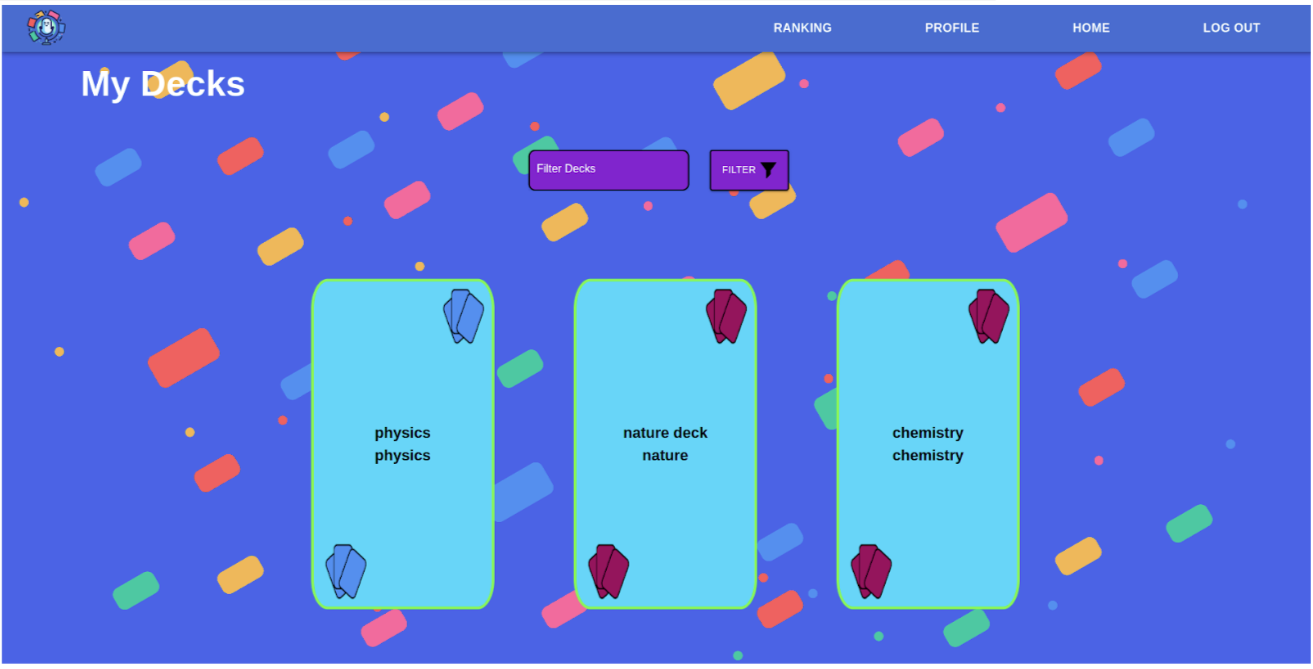
\includegraphics[width=0.9\textwidth]{chapters/chapter_10/images_web/web_my_decks}
    \caption{Widok talii utworzonych przez użytkownika.}
    \label{img:web_my_decks}
\end{figure}


Po przejściu ukazują się wszystkie fiszki w talii. Użytkownik po kliknięciu "Learn" uruchamia trybu uczenia, który pozwala na podzielenie talii na fiszek na zapamiętane i niezapamiętane. "Memorized" to widok w którym widać wszystkie zapamiętane fiszki, a w "Not memorized" znajdują się te niezapamiętane. W "Voice control" są dostępne wszystkie fiszki do podziału, co umożliwia użytkownikowi uruchomienie trybu sterowania na całej dostępnej talii. Opcje oferują użytkownikowi:


\begin{itemize}
    \item Udostępnienie talii;
    \item Reset talii w celu ustawienia wszystkich fiszek jako niezapamiętane;
    \item Usunięcie talii;
    \item Dodanie nowej fiszki;
    \item Zmianę nazwy lub kategorii talii.
\end{itemize}


\begin{figure}[H]
    \centering
    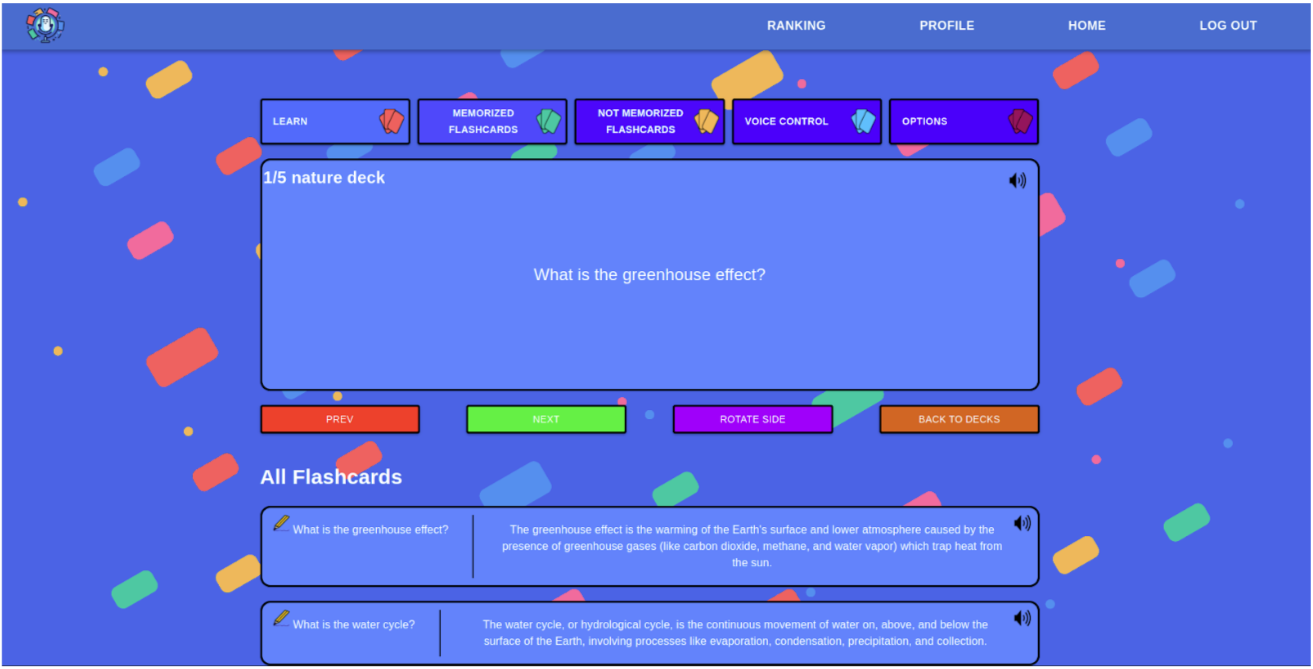
\includegraphics[width=0.9\textwidth]{chapters/chapter_10/images_web/web_deck}
    \caption{Widok talii po jej otworzeniu.}
    \label{img:web_deck}
\end{figure}


\begin{figure}[H]
    \centering
    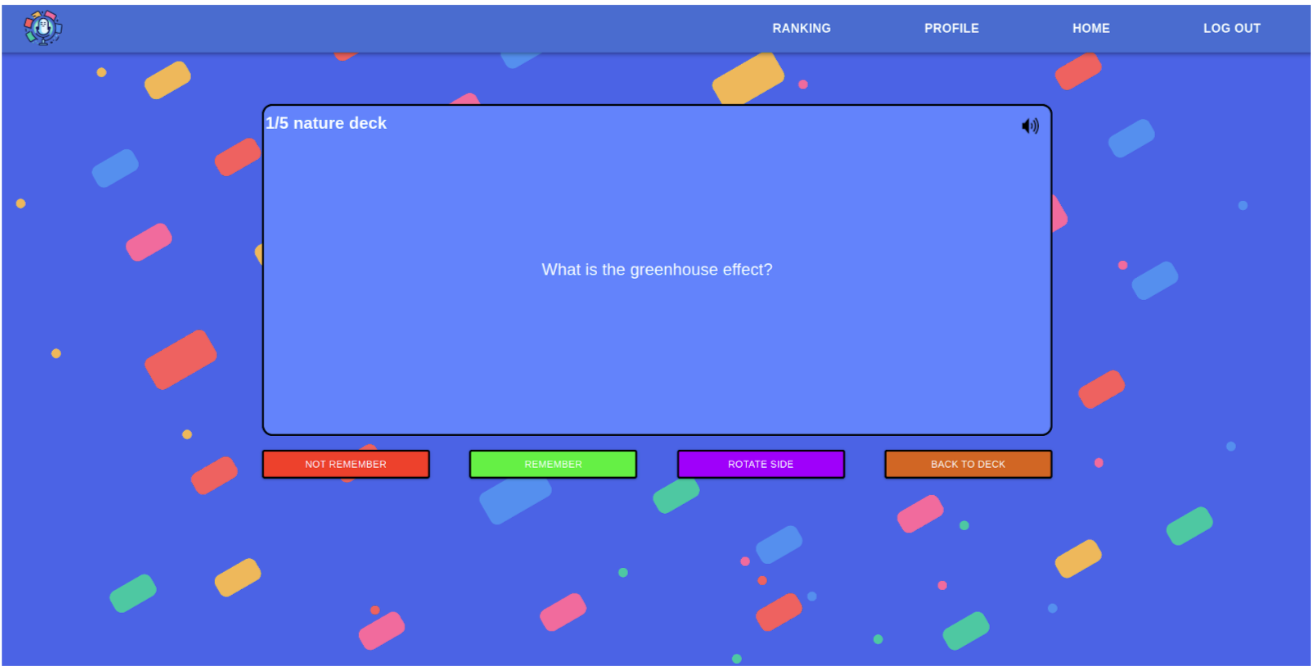
\includegraphics[width=0.9\textwidth]{chapters/chapter_10/images_web/web_learn}
    \caption{Widok podstawowego trybu nauki.}
    \label{img:web_learn}
\end{figure}


\begin{figure}[H]
    \centering
    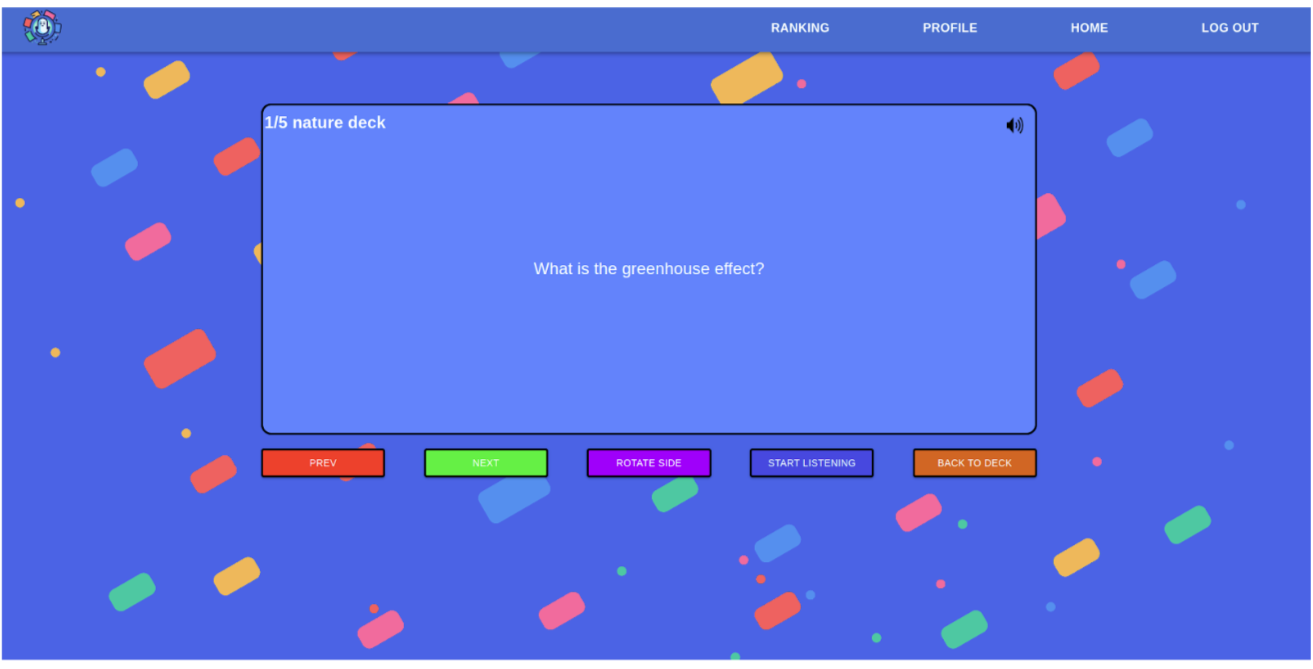
\includegraphics[width=0.9\textwidth]{chapters/chapter_10/images_web/web_voice_1}
    \caption{Widok trybu kontroli głosowej.}
    \label{img:web_voice_1}
\end{figure}


\begin{figure}[H]
    \centering
    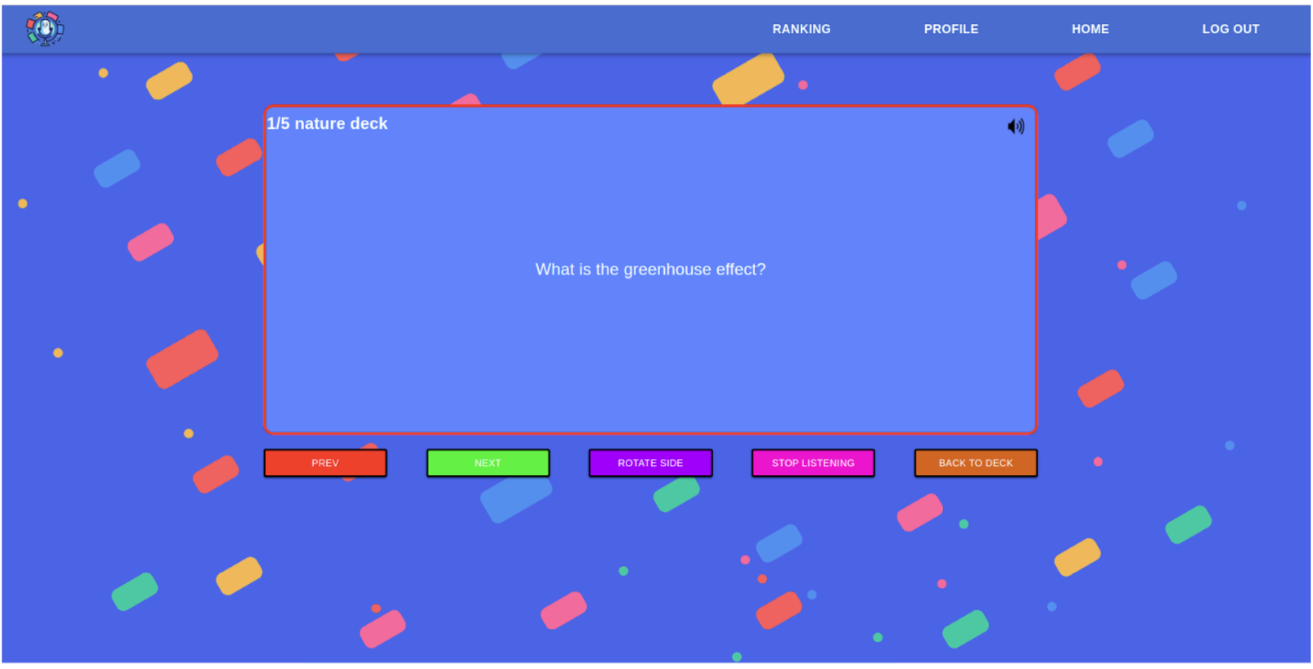
\includegraphics[width=0.9\textwidth]{chapters/chapter_10/images_web/web_voice_2}
    \caption{Widok trybu kontroli głosowej po uruchomieniu.}
    \label{img:web_voice_2}
\end{figure}


\begin{figure}[H]
    \centering
    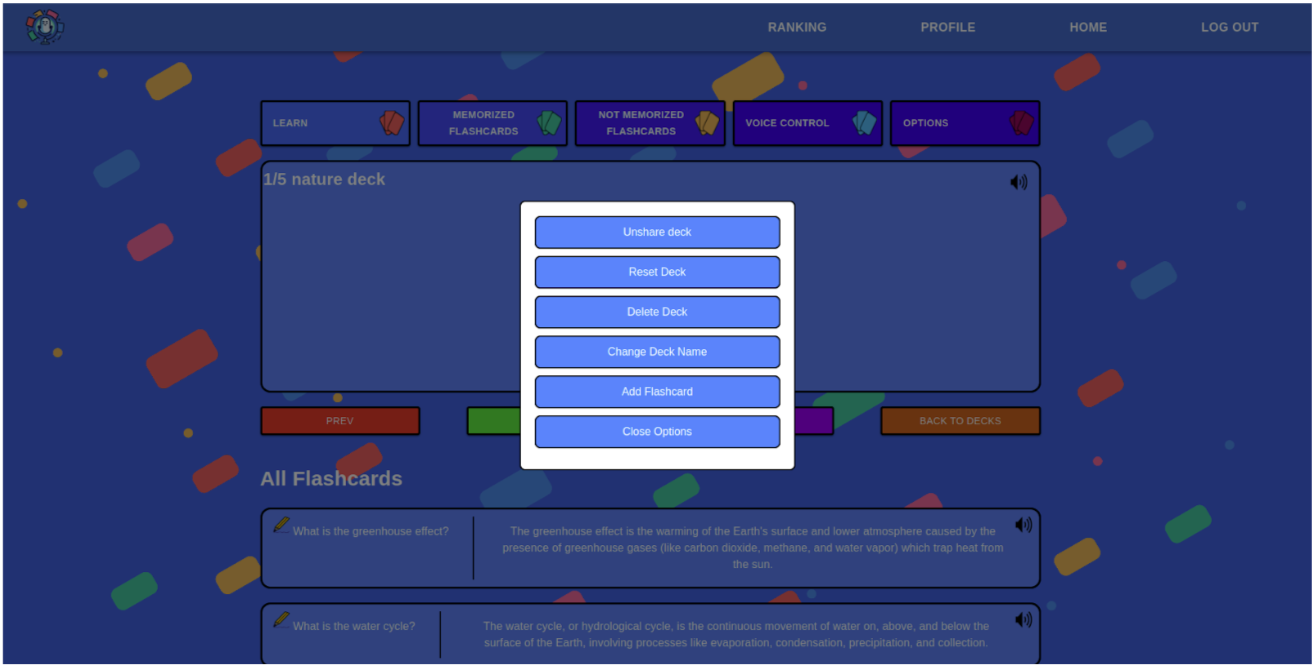
\includegraphics[width=0.9\textwidth]{chapters/chapter_10/images_web/web_settings}
    \caption{Opcje talii.}
    \label{img:web_settings}
\end{figure}


\subsection{"Public decks"}
"Public decks" zawiera wszystkie talie, które zostały zaimportowane z rankingu.


\begin{figure}[H]
    \centering
    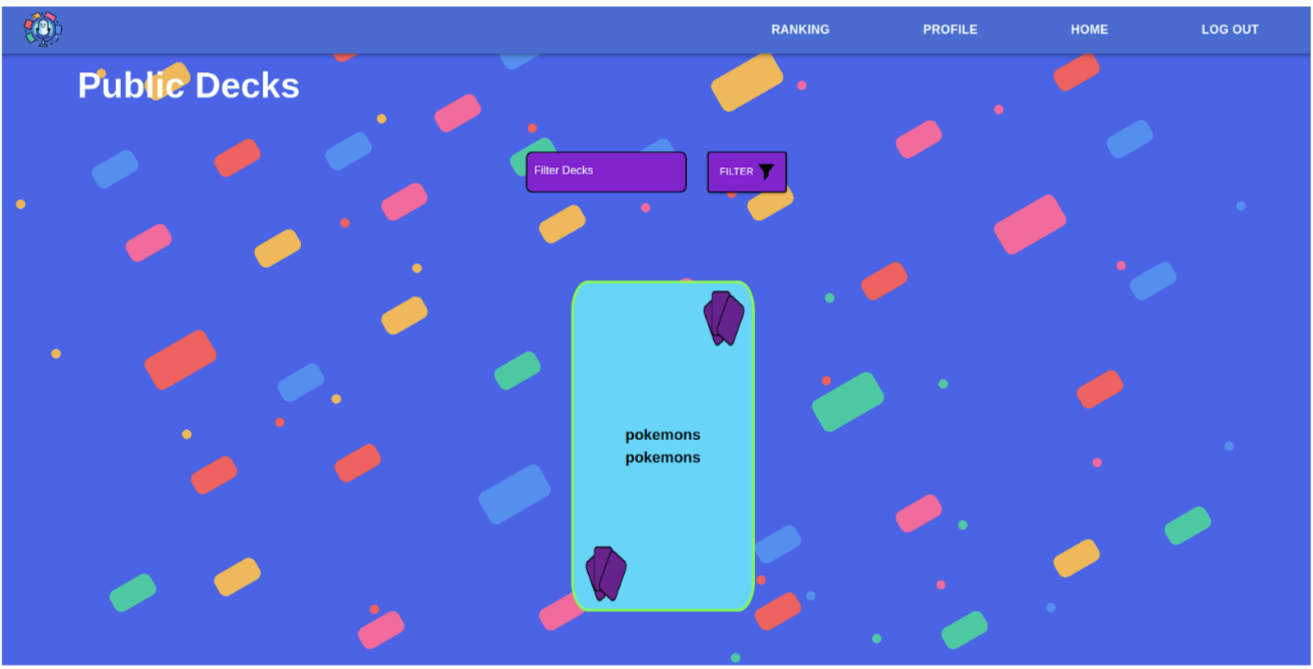
\includegraphics[width=0.9\textwidth]{chapters/chapter_10/images_web/web_public_decks}
    \caption{Widok talii w Public decks.}
    \label{img:web_public_decks}
\end{figure}


\subsection{Ranking użytkowników i talii}
Ranking użytkowników zawiera wszystkie konta, które udostępniły co najmniej jedną talię fiszek. Pozycja w rankingu jest zależna od sumy pobrań wszystkich talii udostępnionych przez użytkownika.


\begin{figure}[H]
    \centering
    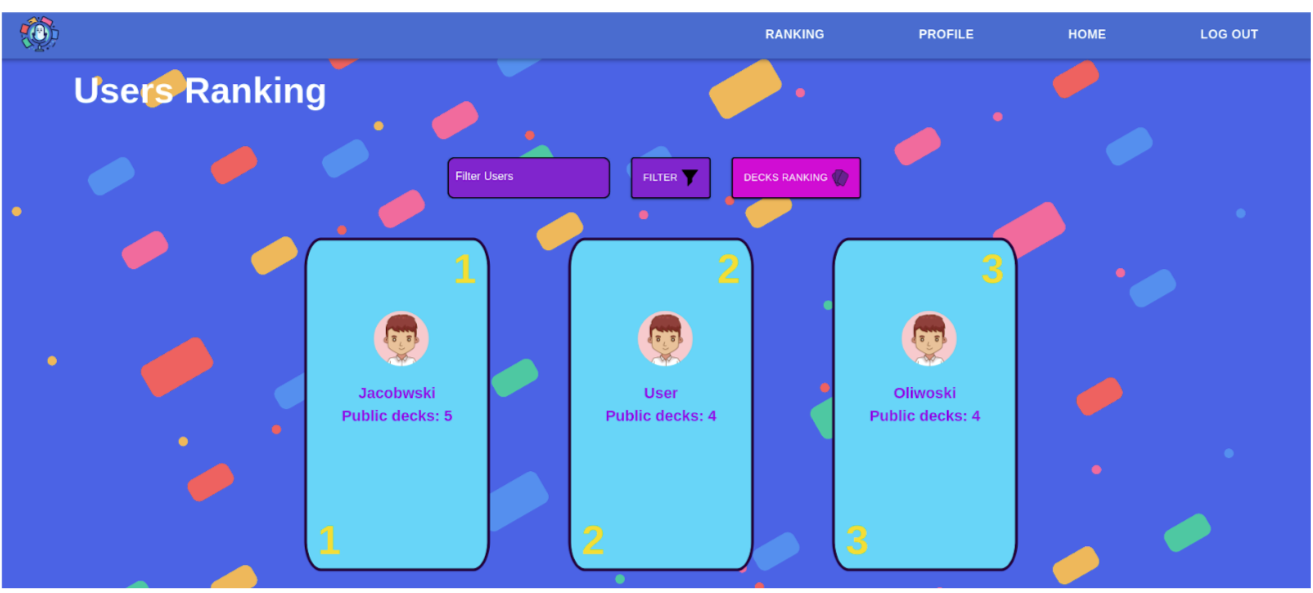
\includegraphics[width=0.9\textwidth]{chapters/chapter_10/images_web/web_user_ranking}
    \caption{Ranking użytkowników.}
    \label{img:web_user_ranking}
\end{figure}


\begin{figure}[H]
    \centering
    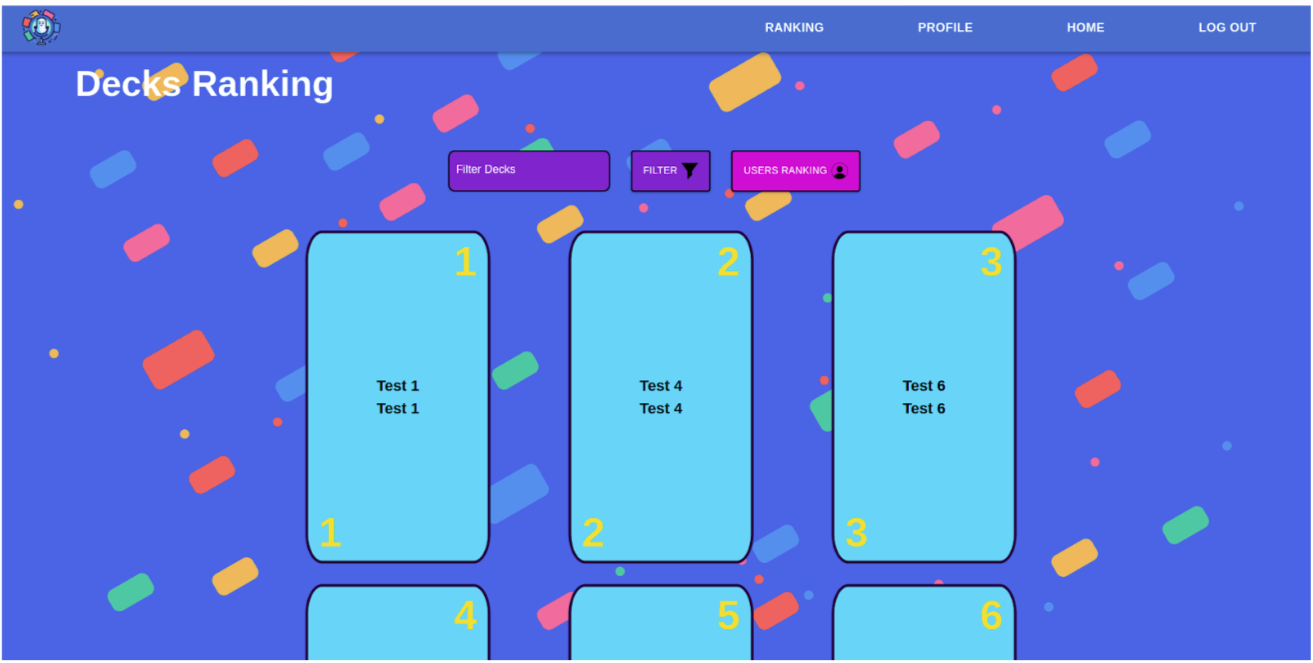
\includegraphics[width=0.9\textwidth]{chapters/chapter_10/images_web/web_decks_ranking}
    \caption{Ranking publicznych talii.}
    \label{img:web_decks_ranking}
\end{figure}


Użytkownik po otworzeniu konkretnej talii ma możliwość obejrzenia jej zawartości. Jeżeli talia spodoba się użytkownikowi, ma on możliwość zaimportowania jej, w ten sposób talia zostanie dodana do "Public decks". Można także zgłosić talię w przypadku gdy zawiera ona wulgaryzmy lub inne nieprzyzwoite wyrażenia. Po zgłoszeniu talii moderator widzi taką talię w zgłoszeniach.

\begin{figure}[H]
    \centering
    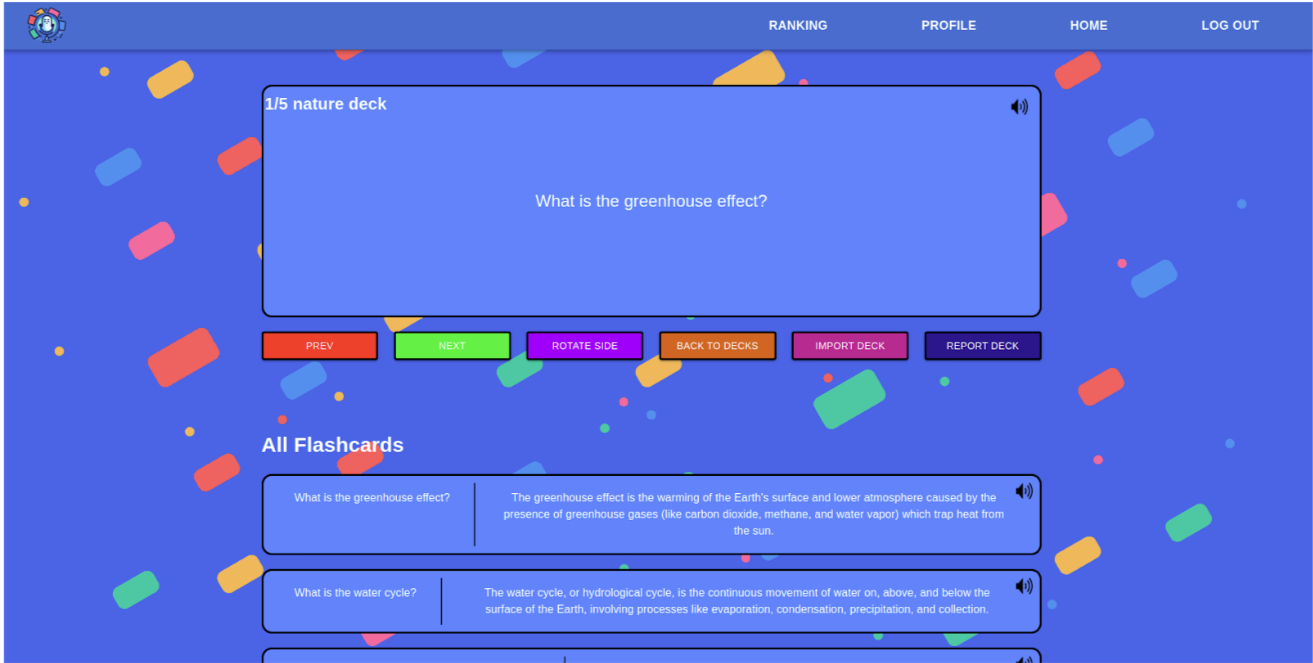
\includegraphics[width=0.9\textwidth]{chapters/chapter_10/images_web/web_public_deck}
    \caption{Widok talii wybranej z rankingu.}
    \label{img:web_public_deck}
\end{figure}

\subsection{Panel moderatora}
Panel moderatora pozwala na usuwanie użytkowników, usuwanie talii, edycję fiszek lub ich usunięcie. Do opcji moderatora mają dostęp tylko osoby z typem konta moderatora lub administratora, w ich przypadku w profilu pojawia się dodatkowy przycisk przekierowujący do panelu.


\begin{figure}[H]
    \centering
    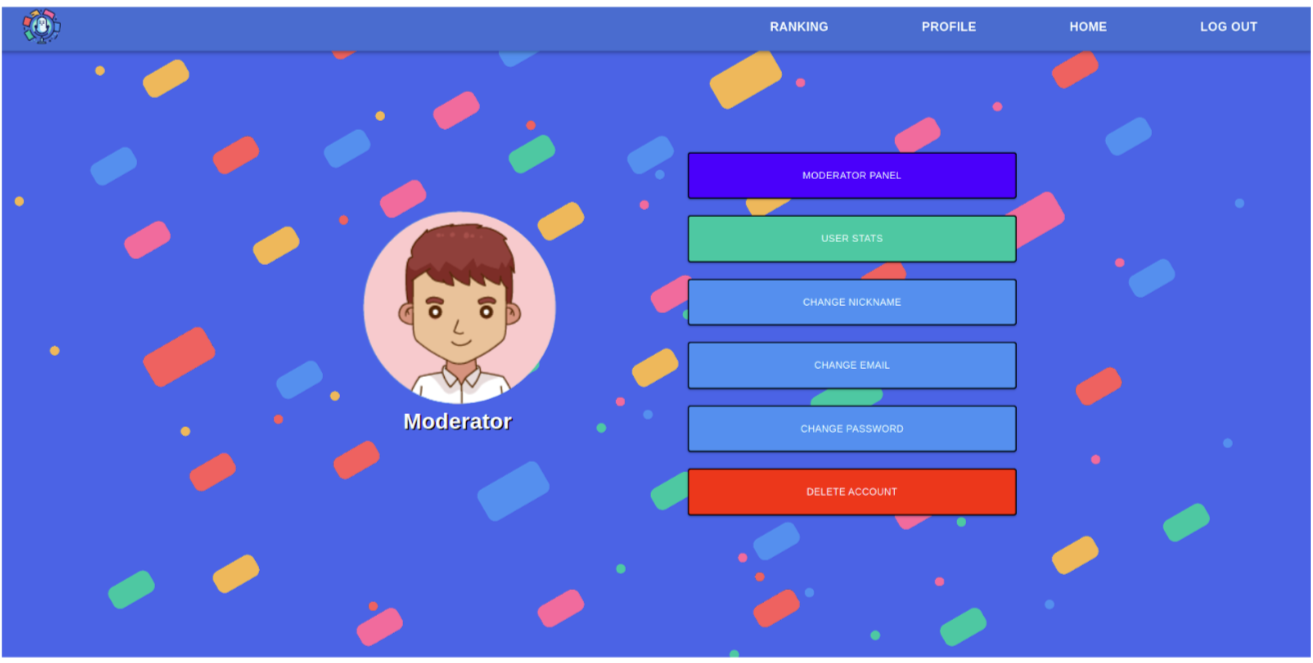
\includegraphics[width=0.9\textwidth]{chapters/chapter_10/images_web/web_moderator_profile}
    \caption{Profil użytkownika konta moderatora.}
    \label{img:web_moderator_profile}
\end{figure}


\begin{figure}[H]
    \centering
    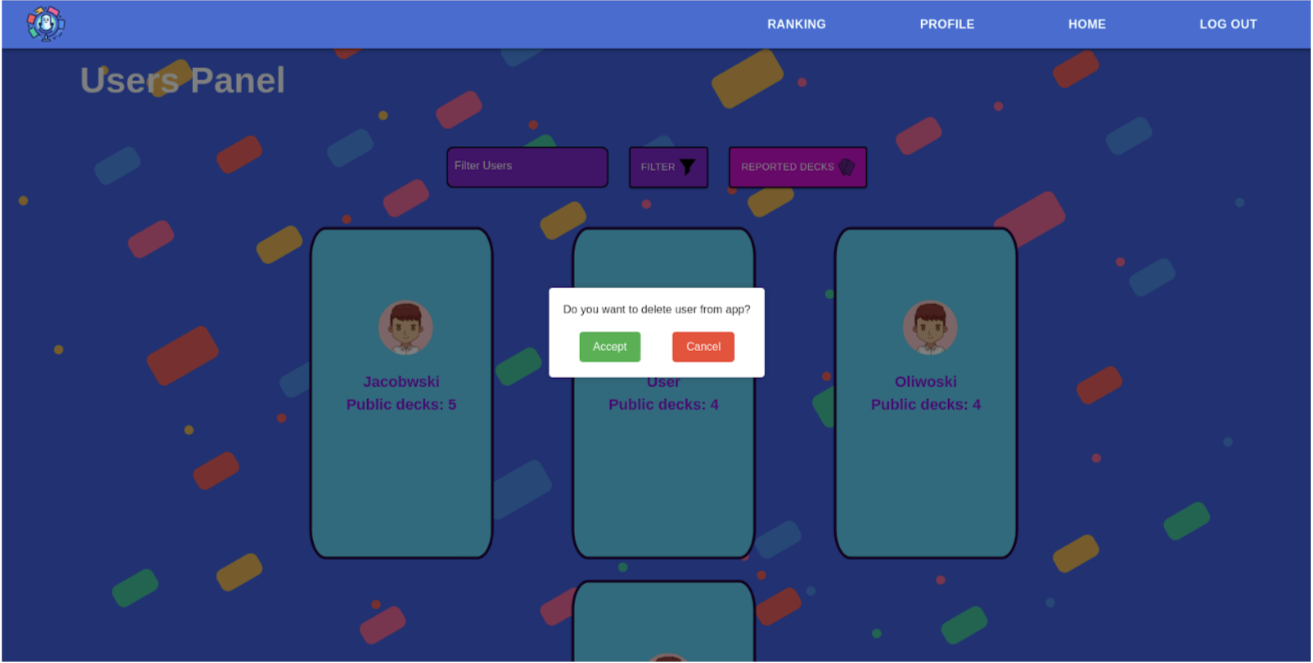
\includegraphics[width=0.9\textwidth]{chapters/chapter_10/images_web/web_moderator_delete_user}
    \caption{Usunięcie użytkownika przez moderatora.}
    \label{img:web_moderator_delete_user}
\end{figure}


\begin{figure}[H]
    \centering
    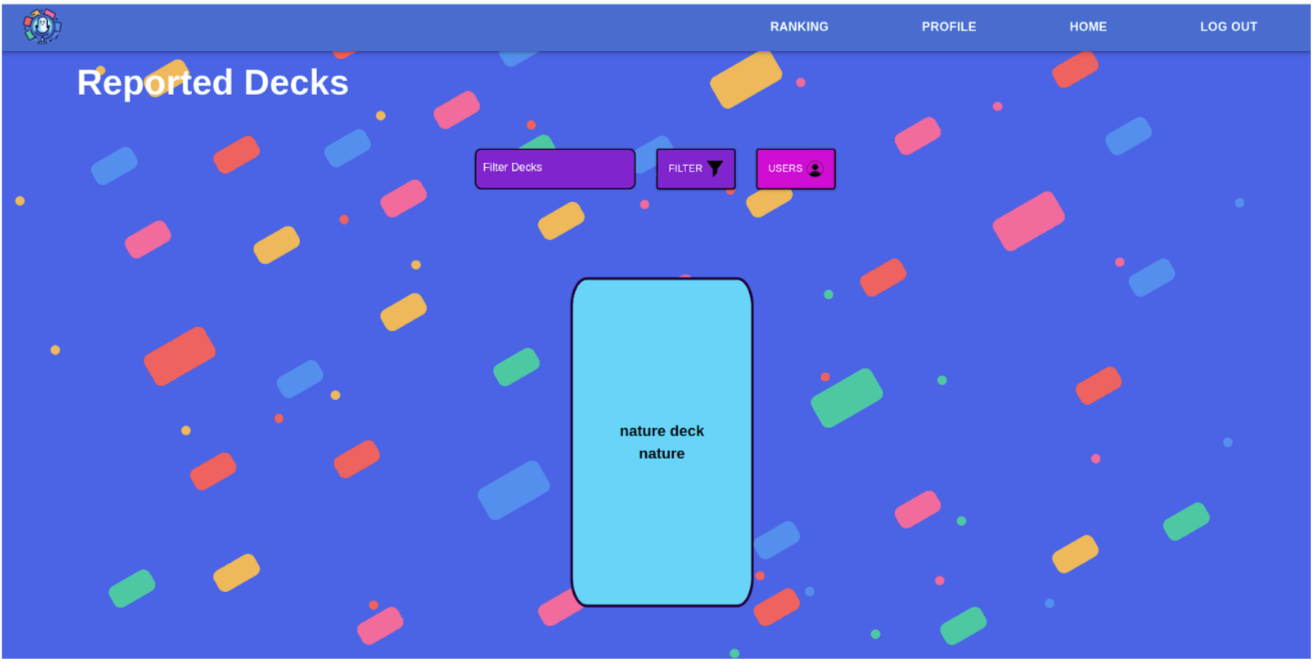
\includegraphics[width=0.9\textwidth]{chapters/chapter_10/images_web/web_reported_decks}
    \caption{Widok zgłoszonych talii.}
    \label{img:web_reported_decks}
\end{figure}


Moderator po otwarciu talii może ją przejrzeć w celu sprawdzenia czy report talii był uzasadniony. W przypadku gdy report talii był nie potrzebny, może usunąć ją z listy zgłoszeń. Jeżeli zgłoszenie było prawidłowe może usunąć talię z aplikacji.


\begin{figure}[H]
    \centering
    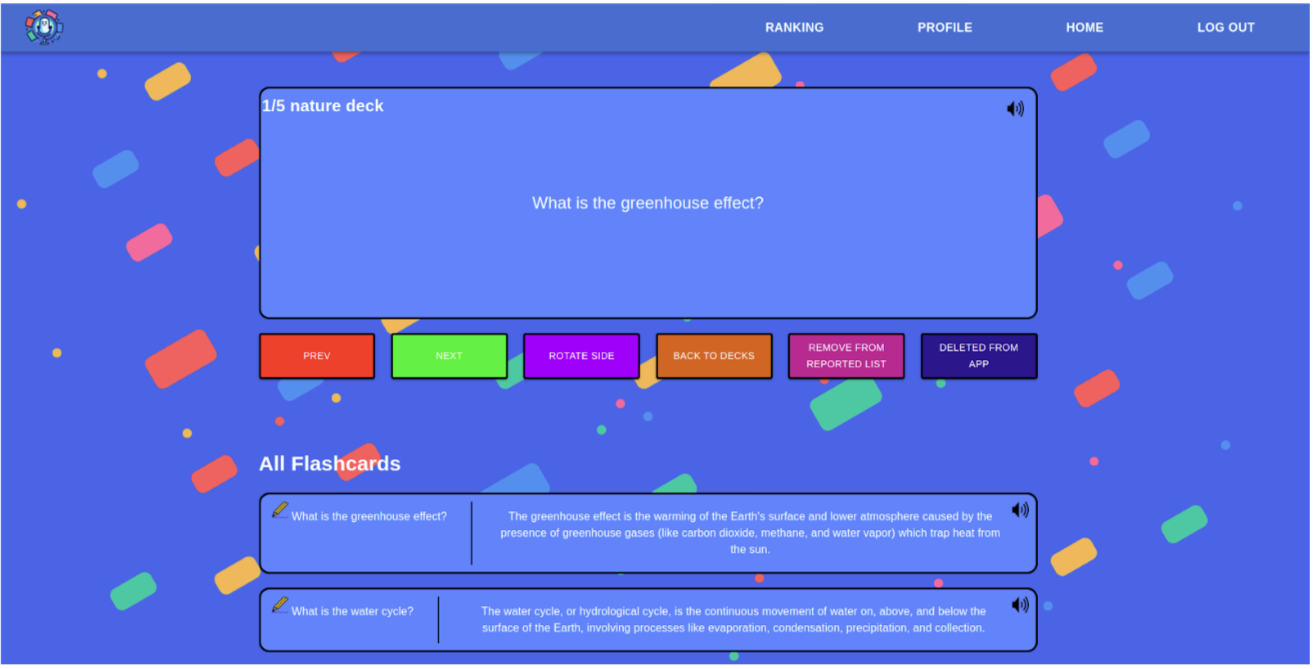
\includegraphics[width=0.9\textwidth]{chapters/chapter_10/images_web/web_reported_deck_2}
    \caption{Widok zgłoszonej talii.}
    \label{img:web_reported_deck_2}
\end{figure}

\newpage
\section{Aplikacja mobilna}
Rozdział przedstawia widoki i działanie aplikacji mobilnej. 


\subsection{Logowanie}
Pierwszym widokiem z perspektywy kodu i użytkownika jest ekran logowania. Aby przejść do aplikacji należy podać prawidłowe dane logowania dla zarejestrowanego wcześniej konta. Aplikacja sprawdza poprawność uzupełnionych pól.


\begin{figure}[H]
    \centering
    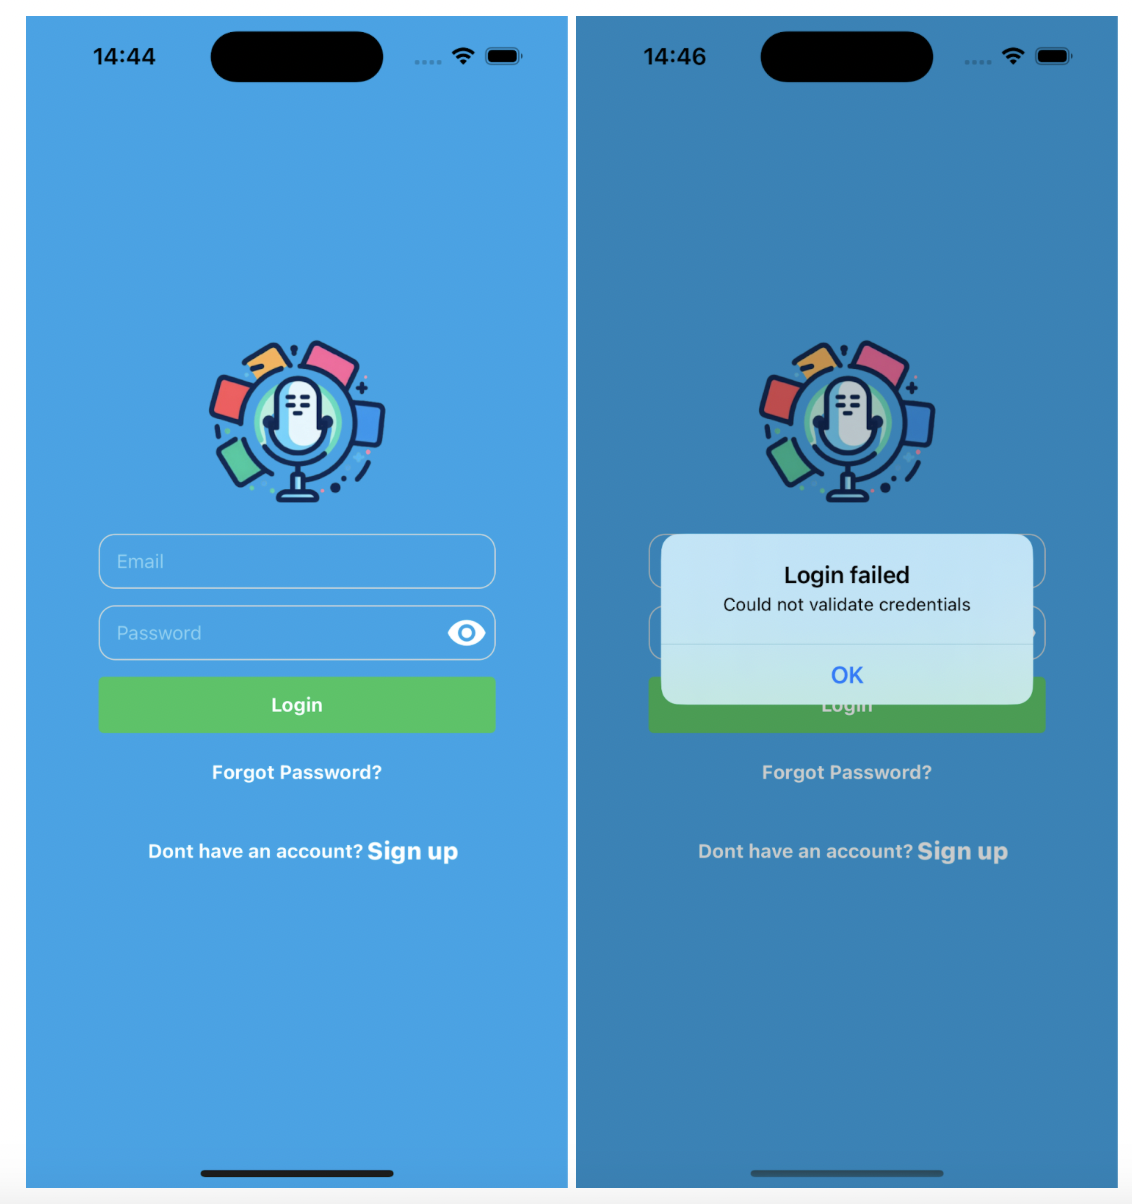
\includegraphics[width=0.9\textwidth]{chapters/chapter_10/images_mobile/mobile_login}
    \caption{Ekran logownia.}
    \label{img:mobile_login}
\end{figure}


\subsection{Rejestracja}
Aby utworzyć konto, którym użytkownik później zaloguje się do aplikacji, należy przejść z widoku logowania do widoku rejestracji. Ta możliwa jest jedynie wtedy, kiedy prawidłowo zostaną uzupełnione pola:
\begin{itemize}
    \item Nazwa użytkownika;
    \item Adres e-mail;
    \item Hasło;
    \item Potwierdź hasło.
\end{itemize}
Aplikacja obsługuje pełną walidację każdego pola i nie pozwoli na utworzenie użytkownika jeżeli podany adres e-mail lub nazwa są zajęte.


\begin{figure}[H]
    \centering
    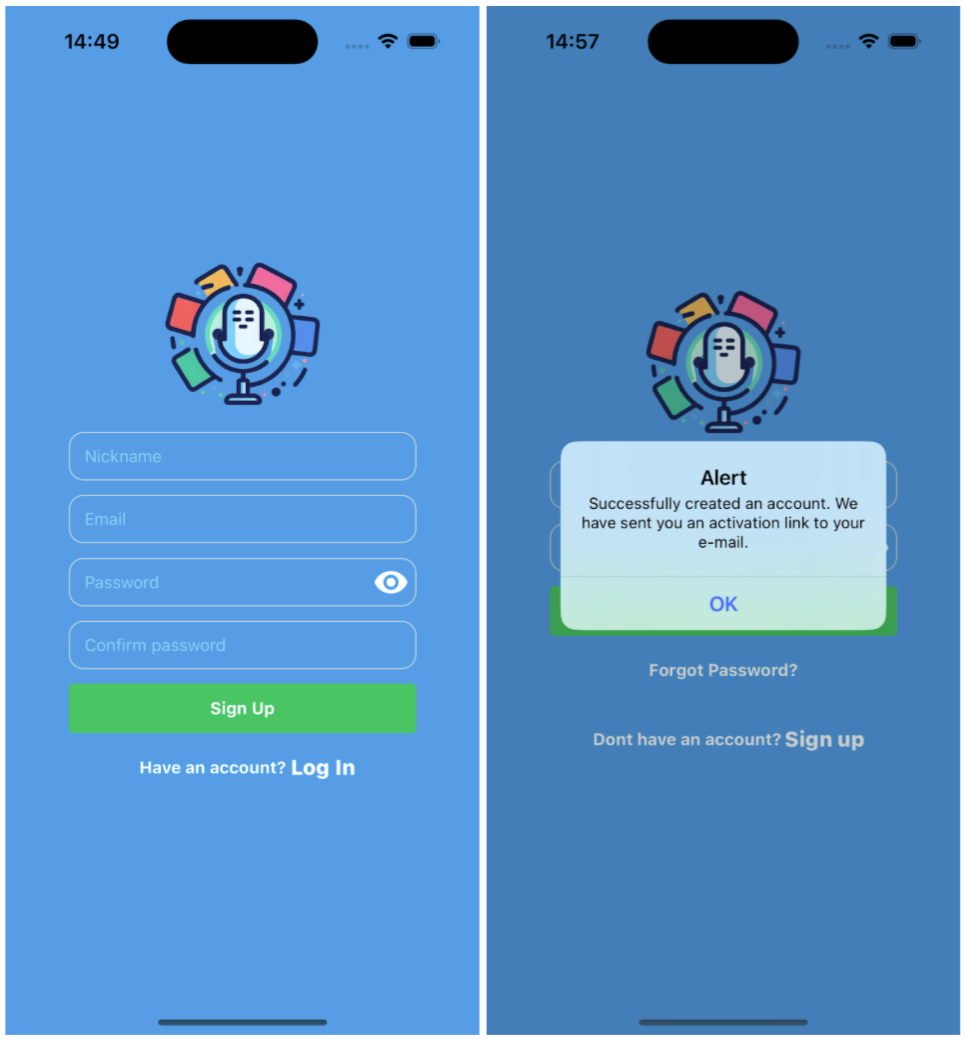
\includegraphics[width=0.9\textwidth]{chapters/chapter_10/images_mobile/mobile_register}
    \caption{Ekran rejestracji.}
    \label{img:mobile_register}
\end{figure}


\subsection{Widok domowy}
Po zalogowaniu użytkownik zostaje przekierowany do widoku domowego. Z tego poziomu możliwe jest:
\begin{itemize}
    \item Utworzenie nowej talii fiszek;
    \item Przejście do widoku talii użytkownika;
    \item Przejście do widoku talii pobranych przez użytkownika.
\end{itemize}


Ponadto, po zalogowaniu użytkownik może w każdej chwili używać dolnego paska nawigacji. Ekran domowy i jemu pochodne znajdują się pod pierwszą ikoną symbolizującą naukę.


\begin{figure}[H]
    \centering
    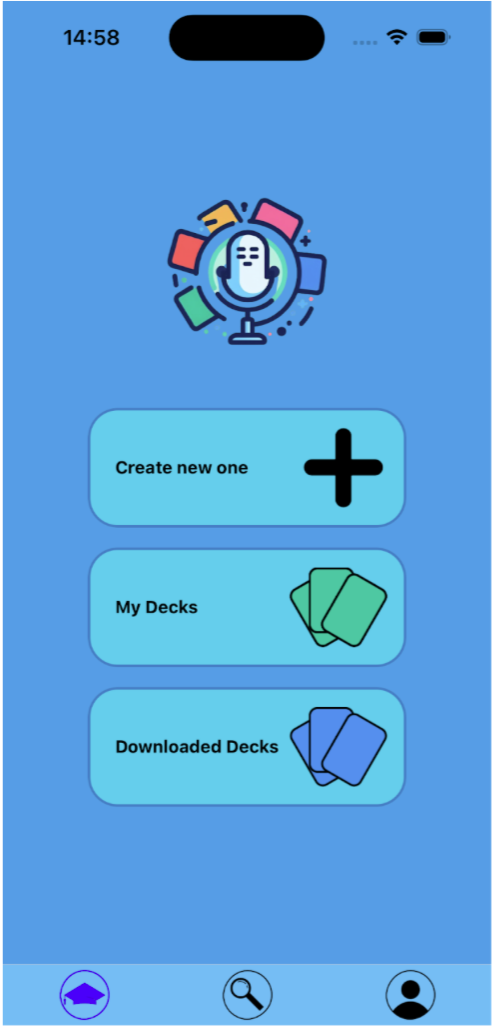
\includegraphics[width=0.4\textwidth]{chapters/chapter_10/images_mobile/mobile_home}
    \caption{Ekran domowy.}
    \label{img:mobile_home}
\end{figure}


\subsection{"My Decks", "My Downloaded Decks" i "Create Deck"}
Po wybraniu przycisku "My Decks" w ekranie domowym, użytkownik zostaje przekierowany do widoku w którym przechowywane są jego talie. Z tego poziomu możliwe jest wyszukanie, wybranie lub utworzenie nowej talii. \\\\
Podobnie w przypadku wybrania opcji “My Downloaded Decks” - tutaj wyświetlone zostaną pobrane talie, wyszukiwanie oraz przycisk nawigujący do rankingu talii publicznych. \\\\
Widok "Create Decks" jest dostępny z ekranu "My Decks" oraz bezpośrednio z ekranu domowego. Aby utworzyć nową talię, wymagane jest podanie jej tytułu i kategorii, oba pola muszą przejść walidacje i nie mogą być puste.


\begin{figure}[H]
    \centering
    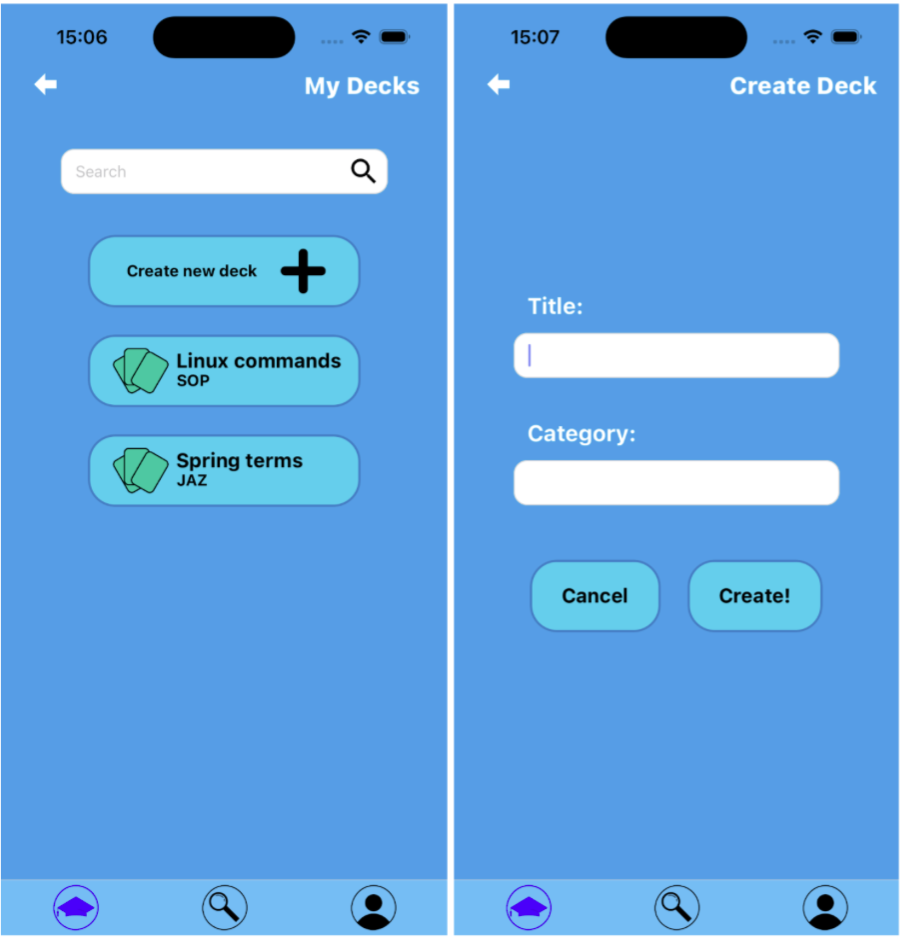
\includegraphics[width=0.8\textwidth]{chapters/chapter_10/images_mobile/mobile_my_decks}
    \caption{Widok "My Decks" i "Create Deck".}
    \label{img:mobile_my_decks}
\end{figure}


\begin{figure}[H]
    \centering
    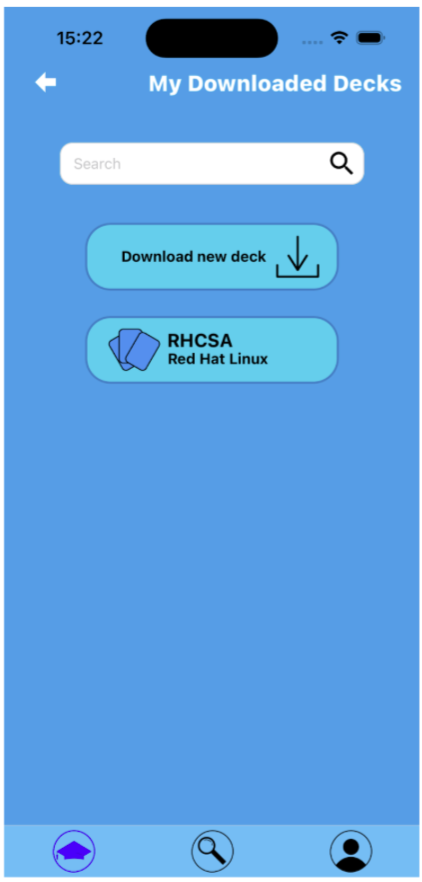
\includegraphics[width=0.4\textwidth]{chapters/chapter_10/images_mobile/mobile_my_decks_2}
    \caption{Widok "My Downloaded Decks".}
    \label{img:mobile_my_decks_2}
\end{figure}


\subsection{"Deck Preview" i "Downloaded Deck Preview"}
Po wybraniu talii z listy w ekranie "My Decks" lub "My downloaded Decks" użytkownik zostaje przekierowany do ekranu podglądu talii. Widok wyświetla:
\begin{itemize}
    \item nazwę talii;
    \item ilość znajdujących się w talii fiszek;
    \item status - "private" lub "public" (widoczne tylko w ekranie "Deck Preview").
\end{itemize}

Ponadto możliwa jest nawigacja do kolejnych widoków:
\begin{itemize}
    \item "Review flashcards";
    \item "Learn with flashcards";
    \item "Voice control";
    \item "Memorized flashcards";
    \item "Unmemorized flashcards";
    \item "Settings".
\end{itemize}

\begin{figure}[H]
    \centering
    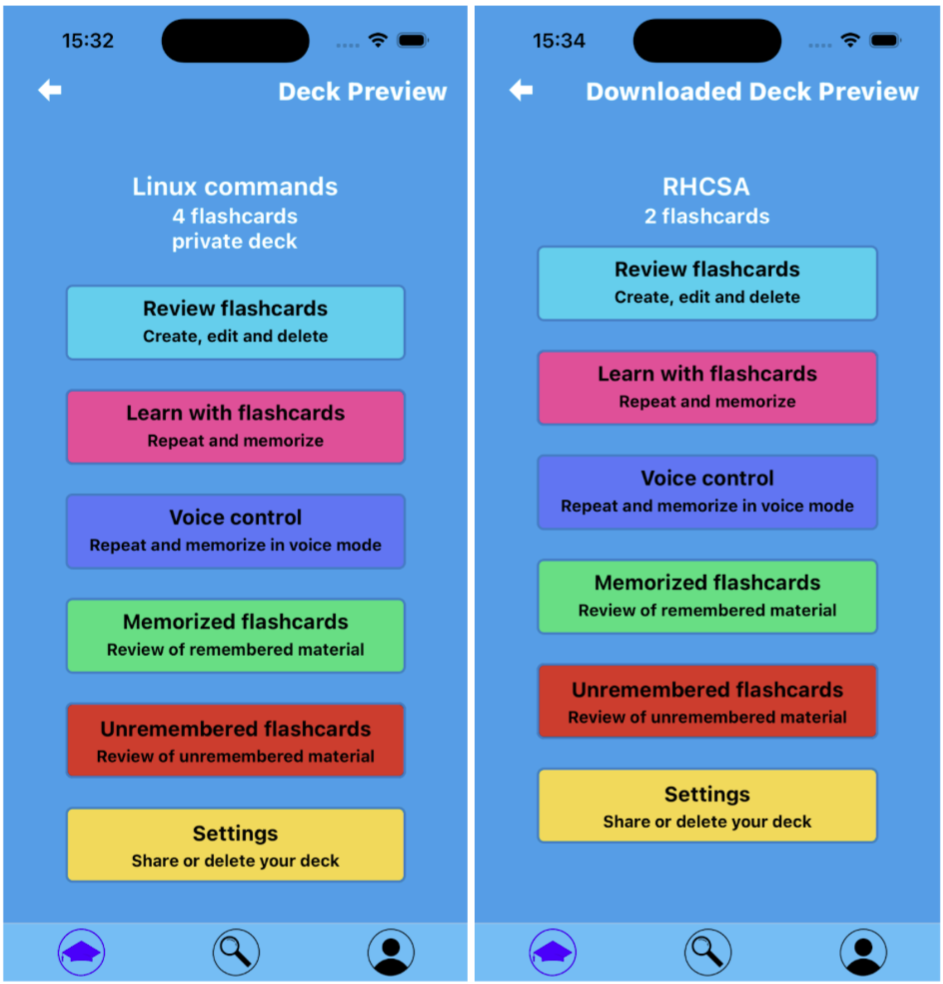
\includegraphics[width=0.8\textwidth]{chapters/chapter_10/images_mobile/mobile_deck_preview}
    \caption{Widok "Deck Preview" i "Downloaded Deck preview".}
    \label{img:mobile_deck_preview}
\end{figure}


\subsection{"Review flashcards"}
Po wybraniu w widoku podglądu talii przycisku "Review flashcards", użytkownik zostanie przeniesiony do podglądu fiszek. W nim wyświetlone są wszystkie fiszki. Funkcjonalności dostępne z tego poziomu to:
\begin{itemize}
    \item utworzenie nowej fiszki za pomocą przycisku “Create new flashcard”'
    \item usunięcie istniejącej fiszki za pomocą przycisku z ikoną kosza;
    \item edycja istniejącej fiszki za pomocą przycisku z ikoną ołówka.
\end{itemize}


\begin{figure}[H]
    \centering
    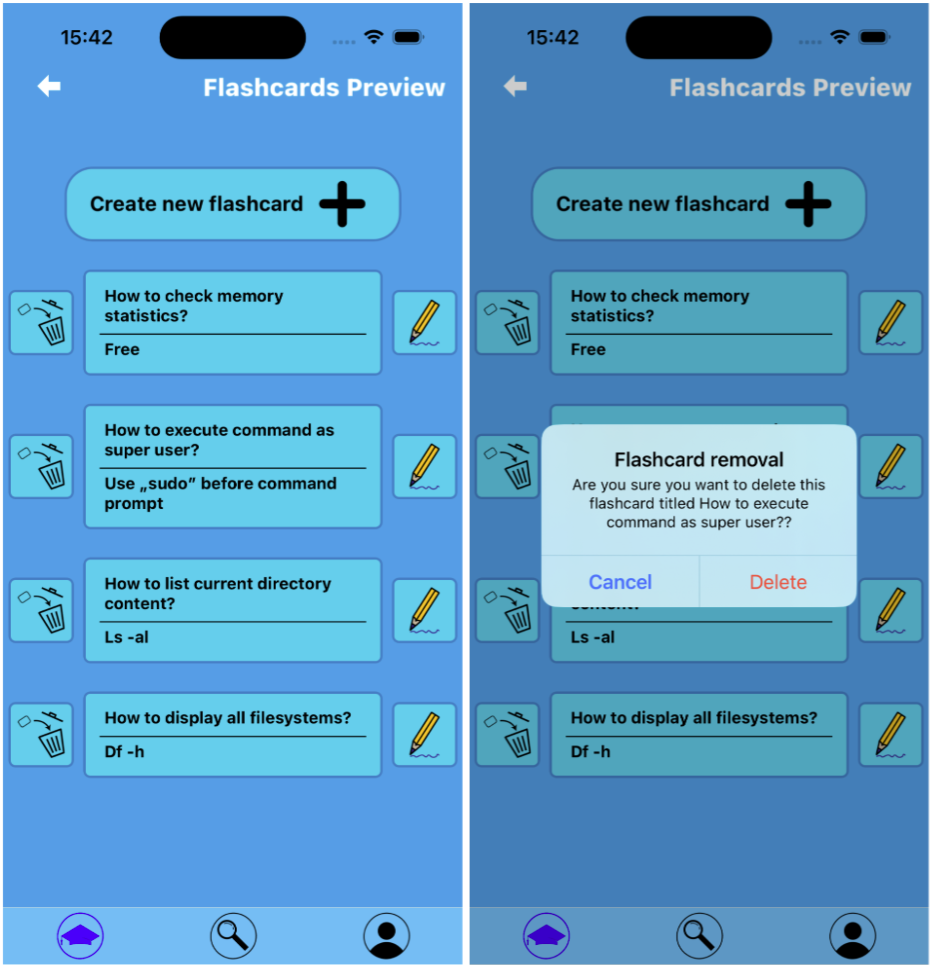
\includegraphics[width=0.9\textwidth]{chapters/chapter_10/images_mobile/mobile_flashcards_preview}
    \caption{Widok "Flashcards Preview" i potwierdzenie usunięcia fiszki.}
    \label{img:mobile_flashcards_preview}
\end{figure}


\subsection{"Create Flashcard" i "Edit Flashcard"}
Po wybraniu opcji edycji lub utworzenia fiszki, użytkownik zostanie przekierowany do odpowiedniego widoku w którym możliwe jest:
\begin{itemize}
    \item uzupełnienie przedniej strony fiszki;
    \item uzupełnienie tylnej strony fiszki;
    \item wygenerowanie treści tylnej strony fiszki na podstawie treści strony przedniej;
    \item zaakceptowanie lub odrzucenie wygenerowanej treści (po naciśnięciu przycisku generowania).
\end{itemize}


\begin{figure}[H]
    \centering
    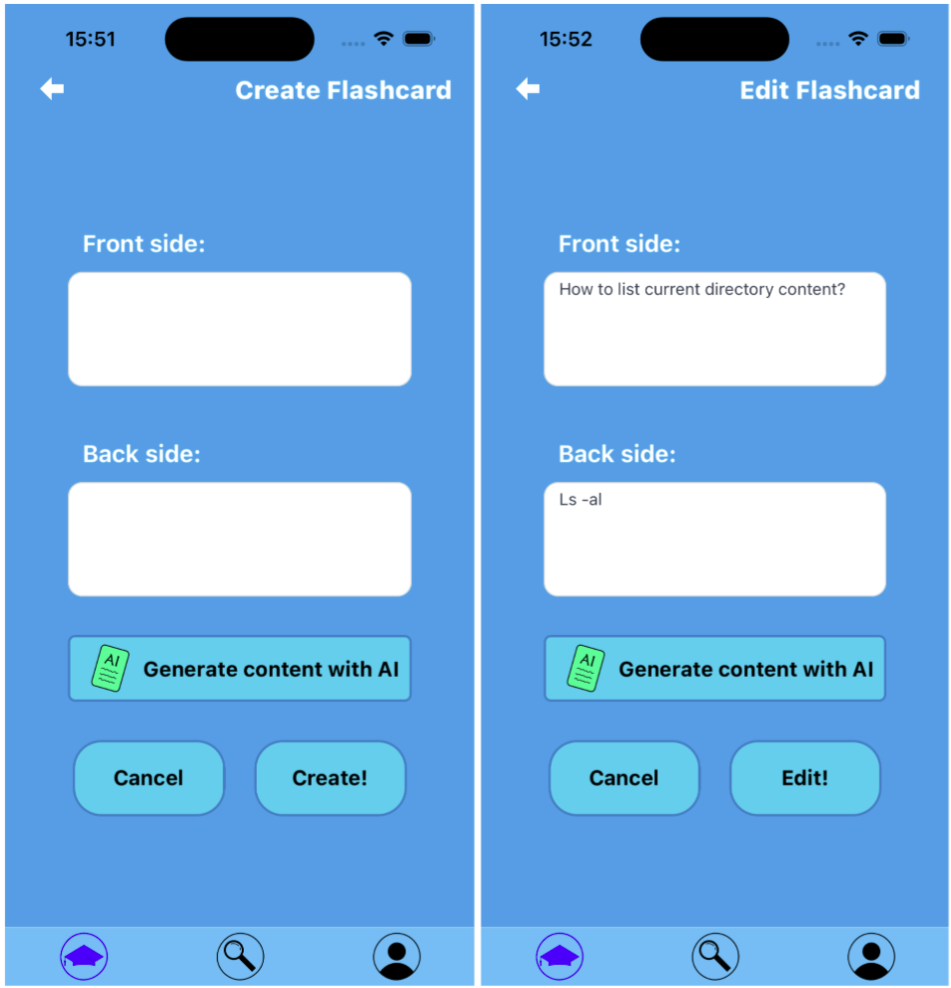
\includegraphics[width=0.9\textwidth]{chapters/chapter_10/images_mobile/mobile_create_flashcards}
    \caption{Widoki "Create Flashcard" i "Edit Flashcard".}
    \label{img:mobile_create_flashcards}
\end{figure}


\begin{figure}[H]
    \centering
    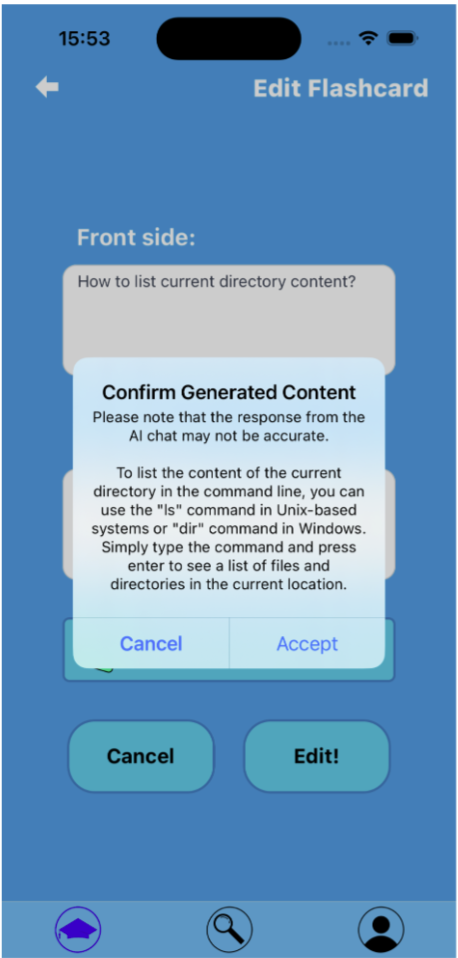
\includegraphics[width=0.5\textwidth]{chapters/chapter_10/images_mobile/mobile_chat}
    \caption{Podgląd treści wygenerowanej przez AI.}
    \label{img:mobile_chat}
\end{figure}


\subsection{"Learn with flashcards"}
Podstawowy tryb nauki, w nim wyświetlane są kolejno fiszki z odkrytymi zagadnieniami. Po naciśnięciu w fiszkę, użytkownik może podejrzeć jej definicje. Przejście do kolejnej fiszki odbywa się po odznaczeniu bieżącej fiszki jako tej zapamiętanej za pomocą zielonego przycisku lub jako niezapamiętanej za pomocą przycisku czerwonego.


\begin{figure}[H]
    \centering
    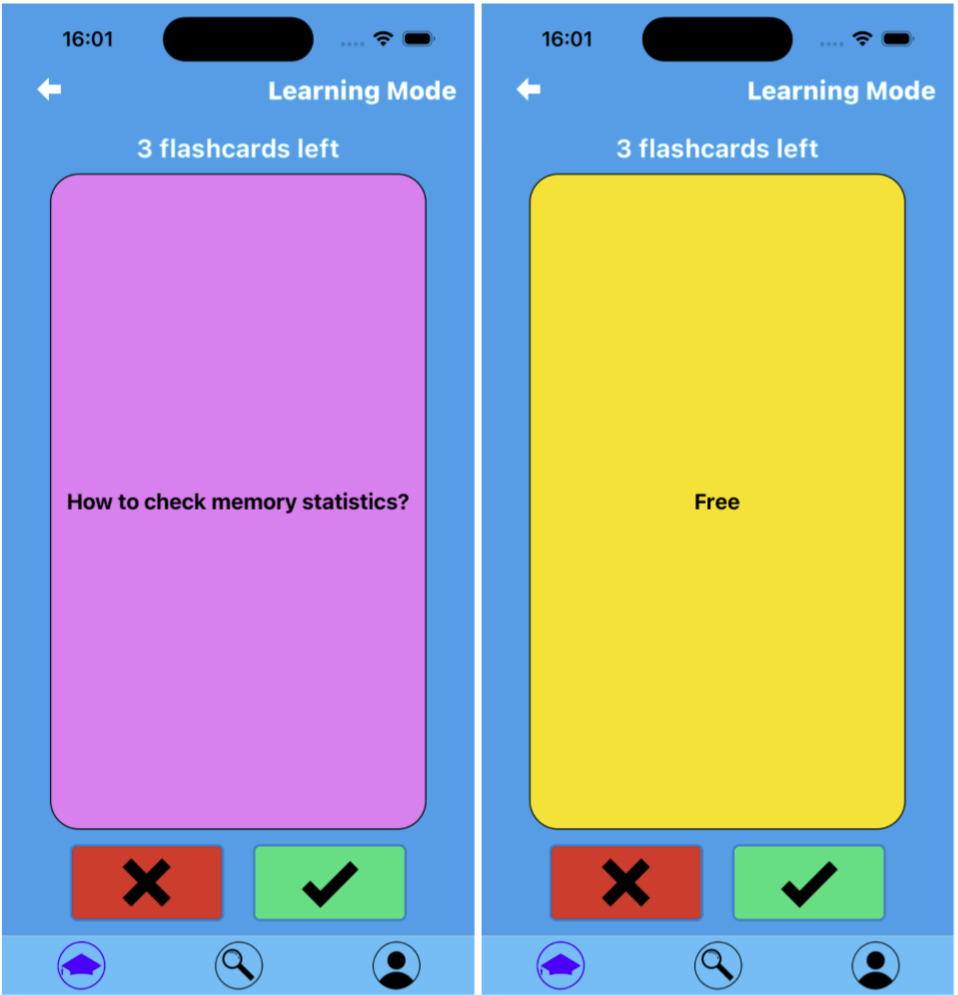
\includegraphics[width=0.9\textwidth]{chapters/chapter_10/images_mobile/mobile_learn}
    \caption{Podstawowy tryb nauki.}
    \label{img:mobile_learn}
\end{figure}


\begin{figure}[H]
    \centering
    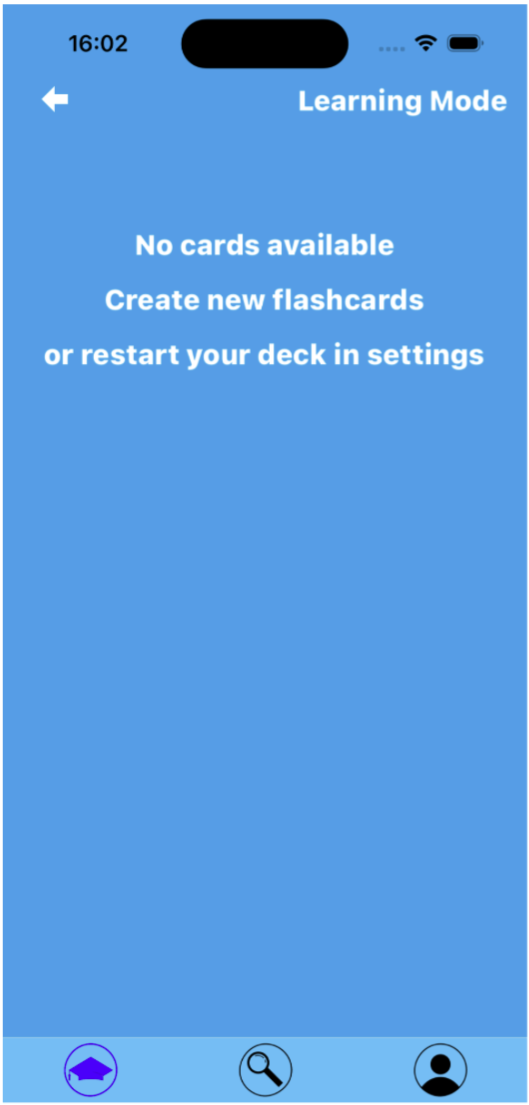
\includegraphics[width=0.5\textwidth]{chapters/chapter_10/images_mobile/mobile_learn_2}
    \caption{Widok w przypadku kiedy talia jest pusta lub wszystkie fiszki są oznaczone jako zapamiętane.}
    \label{img:mobile_learn_2}
\end{figure}


\subsection{"Voice control"}
Tryb nauki z obsługą głosową. Widok pozwala na przeglądanie talii za pomocą komend głosowych po naciśnięciu przycisku z ikoną mikrofonu.

\begin{figure}[H]
    \centering
    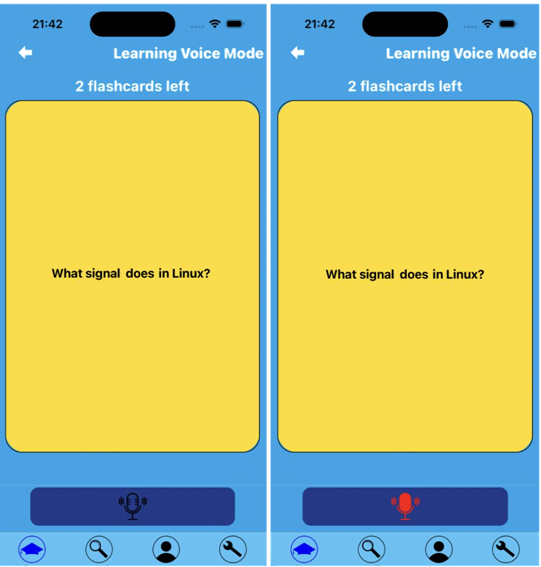
\includegraphics[width=0.9\textwidth]{chapters/chapter_10/images_mobile/mobile_voice_control}
    \caption{Widok głosowego trybu nauki.}
    \label{img:mobile_voice_control}
\end{figure}

\subsection{"Memorized flashcards" i "Unmemorized flashcards"}
Widoki podglądowe dla fiszek oznaczonych jako zapamiętane i niezapamiętane. Poza możliwością przeglądania fiszek, możliwe jest odsłuchanie ich treści.

\begin{figure}[H]
    \centering
    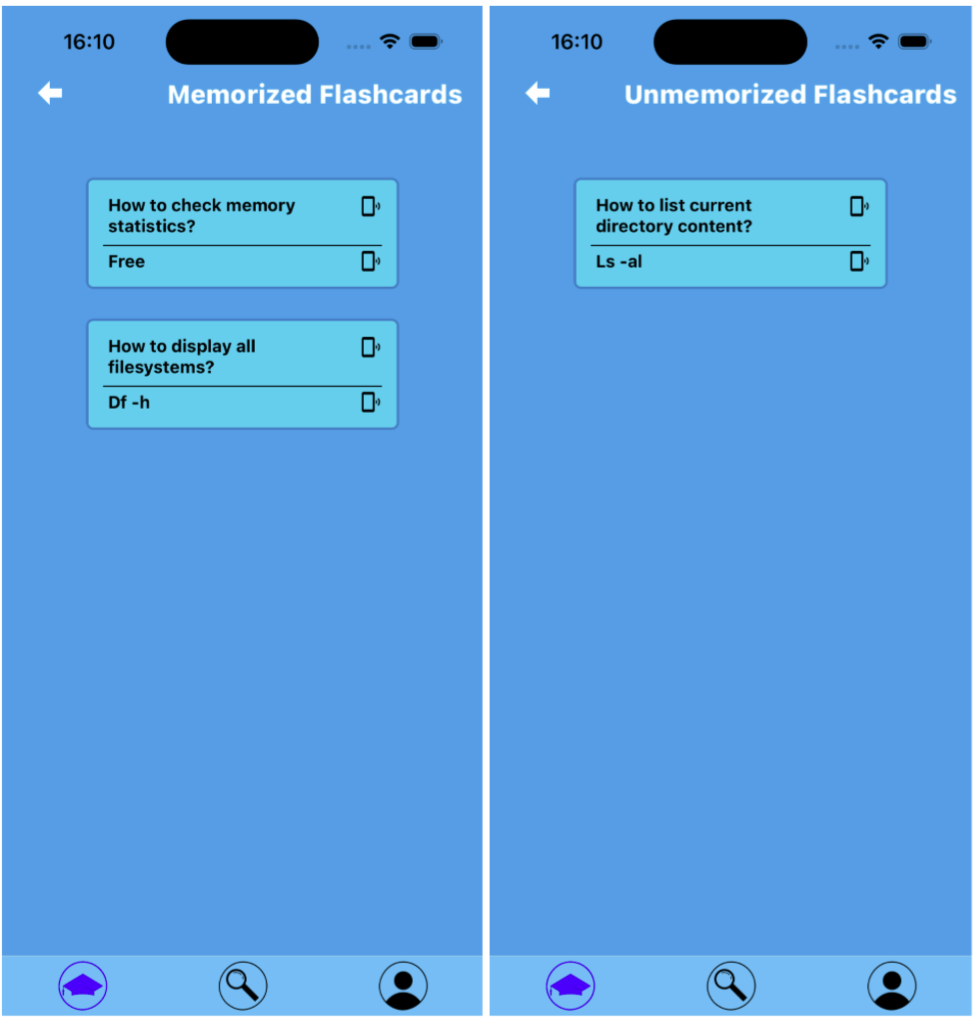
\includegraphics[width=0.9\textwidth]{chapters/chapter_10/images_mobile/mobile_memorized}
    \caption{Widoki "Memorized flashcards" i "Unmemorized flashcards".}
    \label{img:mobile_memorized}
\end{figure}

\subsection{"Settings"}
Widok opcji danej talii. Z tego poziomu jest możliwe:
\begin{itemize}
    \item edycja nazwy i kategorii talii (widok bliźniaczy do "Create Deck");
    \item usunięcie talii permanentnie;
    \item udostępnienie talii publicznie lub cofnięcie udostępnienia (opcja niedostępna dla talii bez fiszek oraz talii pobranych z rankingu);
    \item restart talii, czyli oznaczenie wszystkich fiszek jako niezapamiętanych.
\end{itemize}


\begin{figure}[H]
    \centering
    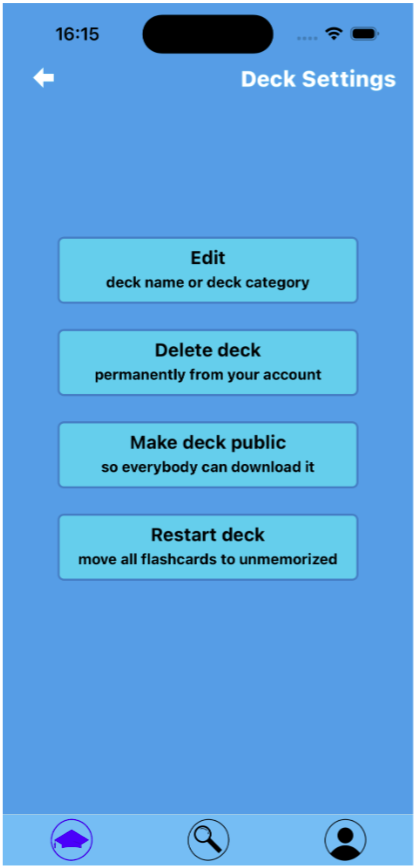
\includegraphics[width=0.5\textwidth]{chapters/chapter_10/images_mobile/mobile_deck_settings}
    \caption{Widok "Deck Settings".}
    \label{img:mobile_deck_settings}
\end{figure}


\subsection{"Public decks" i "Users ranking"}
Widok "Public decks" jest dostępny z poziomu dolnego paska nawigacji pod ikoną lupy. Wyświetla listę wszystkich talii udostępnionych publicznie, posegregowanych po liczbie pobrań. Umożliwia przełączenie na widok rankingu użytkowników posegregowanych po liczbie udostępnionych talii. W obu zakładkach możliwe jest wyszukanie zarówno talii jak i użytkowników.


\begin{figure}[H]
    \centering
    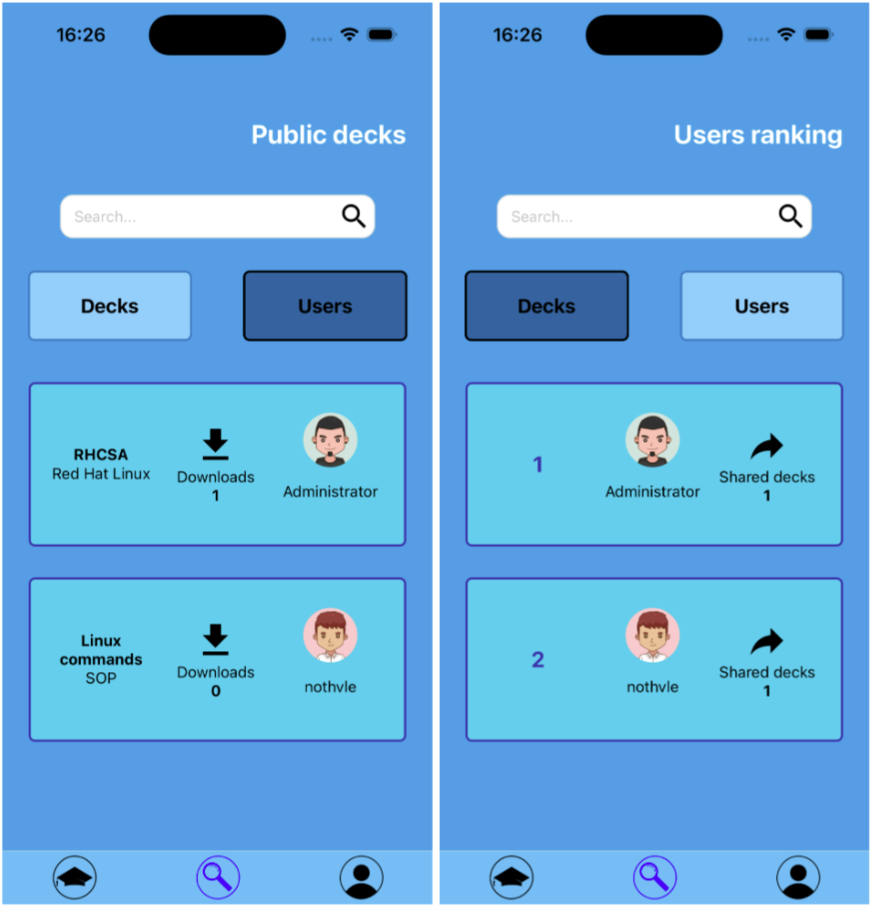
\includegraphics[width=0.9\textwidth]{chapters/chapter_10/images_mobile/mobile_ranking}
    \caption{Widok "Public decks" i "Users ranking".}
    \label{img:mobile_ranking}
\end{figure}


\subsection{Podgląd talii publicznej}
Z poziomu rankingu talii publicznych możliwe jest wybranie interesującej dla użytkownika pozycji. Następuje wtedy przeniesieniu do widoku podglądu talii i jej fiszek. Dostępne funkcjonalności to pobranie talii lub zgłoszenie jej moderatorowi.


\begin{figure}[H]
    \centering
    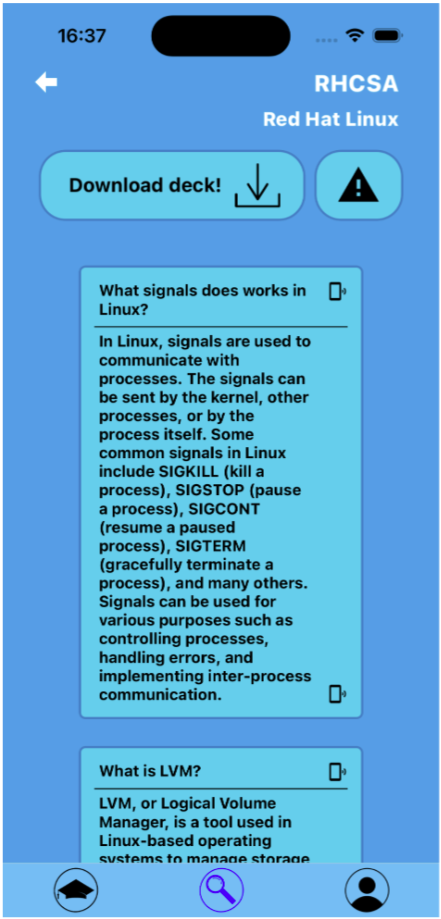
\includegraphics[width=0.5\textwidth]{chapters/chapter_10/images_mobile/mobile_public_deck}
    \caption{Podgląd talii udostępnionej publicznie.}
    \label{img:mobile_public_deck}
\end{figure}

\subsection{Podgląd innego użytkownika}
Możliwe jest podejrzenie innego konta użytkownika poprzez wybranie go z rankingu. Widok zawiera podstawowe informacje oraz udostępnione talie.


\begin{figure}[H]
    \centering
    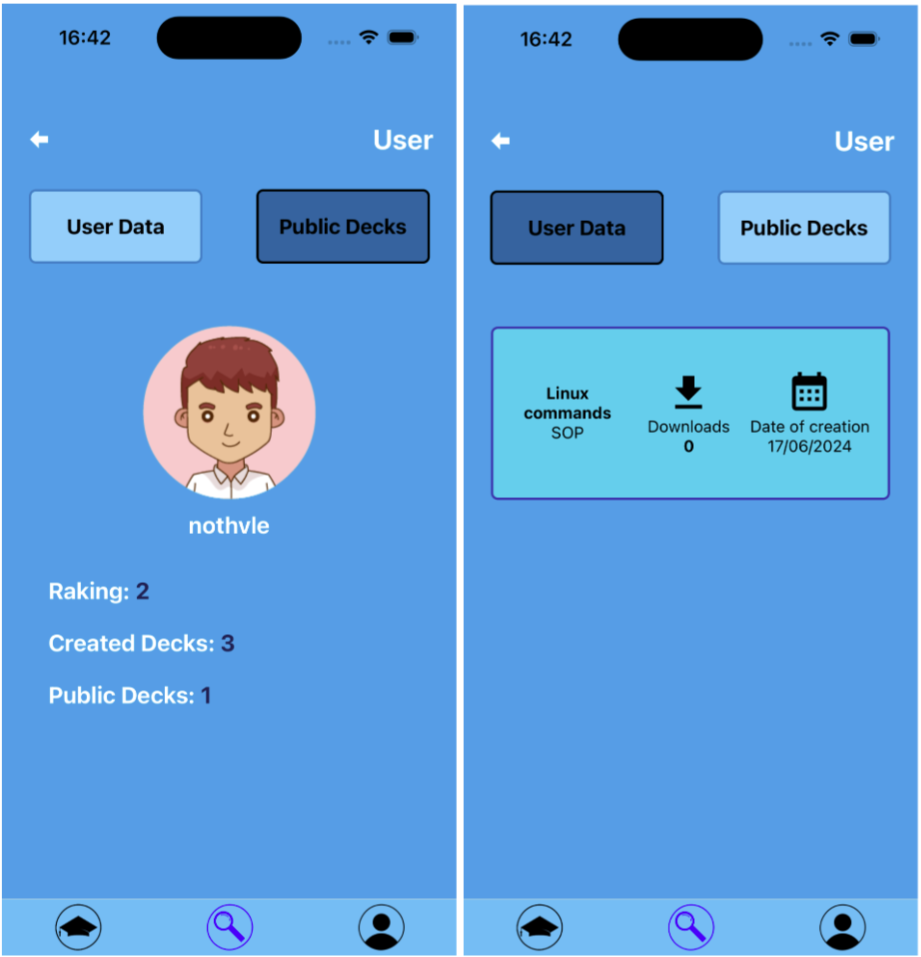
\includegraphics[width=0.9\textwidth]{chapters/chapter_10/images_mobile/mobile_other_user}
    \caption{Podgląd użytkownika i udostępnionych przez niego talii.}
    \label{img:mobile_other_user}
\end{figure}


\subsection{Profil}
Widok profilu jest dostępny z poziomu dolnego paska nawigacji pod ikoną przedstawiającą sylwetkę. W profilu widoczne są:
\begin{itemize}
    \item Informacje o zalogowanym użytkowniku;
    \item Możliwość zmiany adresu e-mail;
    \item Możliwość zmiany hasła;
    \item Możliwość zmiany motywu aplikacji na ciemny;
    \item Możliwość usunięcia konta;
    \item Możliwość wylogowania.
\end{itemize}


\begin{figure}[H]
    \centering
    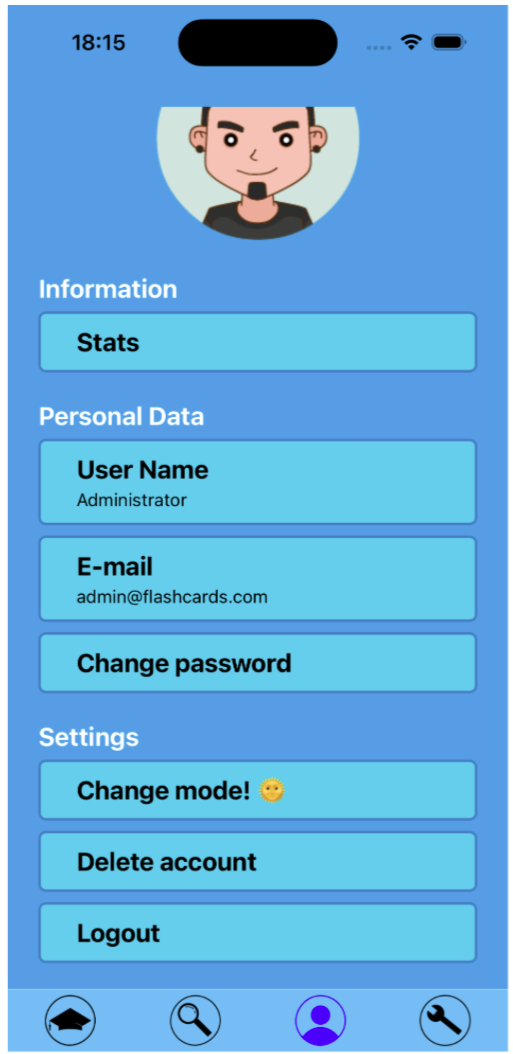
\includegraphics[width=0.5\textwidth]{chapters/chapter_10/images_mobile/mobile_profile}
    \caption{Widok profilu użytkownika.}
    \label{img:mobile_profile}
\end{figure}


\subsection{Widok narzędzi moderatora}
Widok jest dostępny jedynie dla użytkowników wyznaczonych do roli moderatorów i administratorów. Pozwala na zarządzanie pozostałymi użytkownikami oraz zgłoszonymi taliami.


\begin{figure}[H]
    \centering
    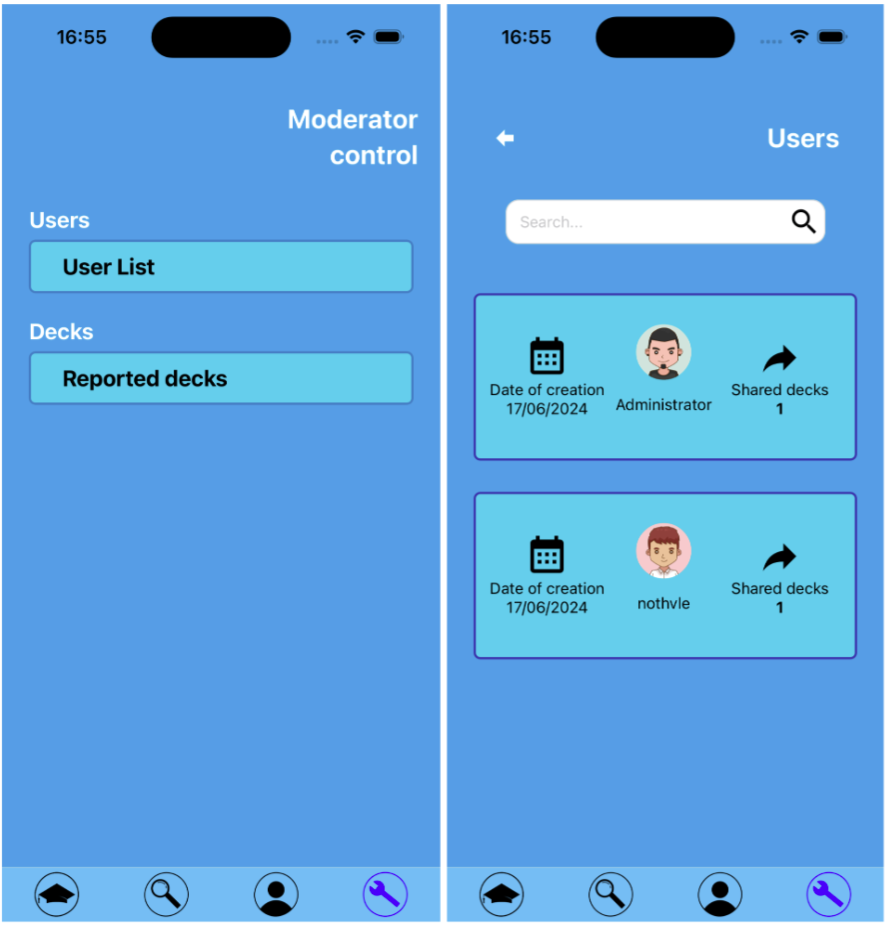
\includegraphics[width=0.9\textwidth]{chapters/chapter_10/images_mobile/moderator_panel}
    \caption{Widok panelu moderatora.}
    \label{img:moderator_panel}
\end{figure}


\subsection{Ciemny motyw aplikacji}
Ciemny motyw jest dostępny w panelu użytkownika. Po jego przełączeniu zmienia się gama kolorów aplikacji.

\begin{figure}[H]
    \centering
    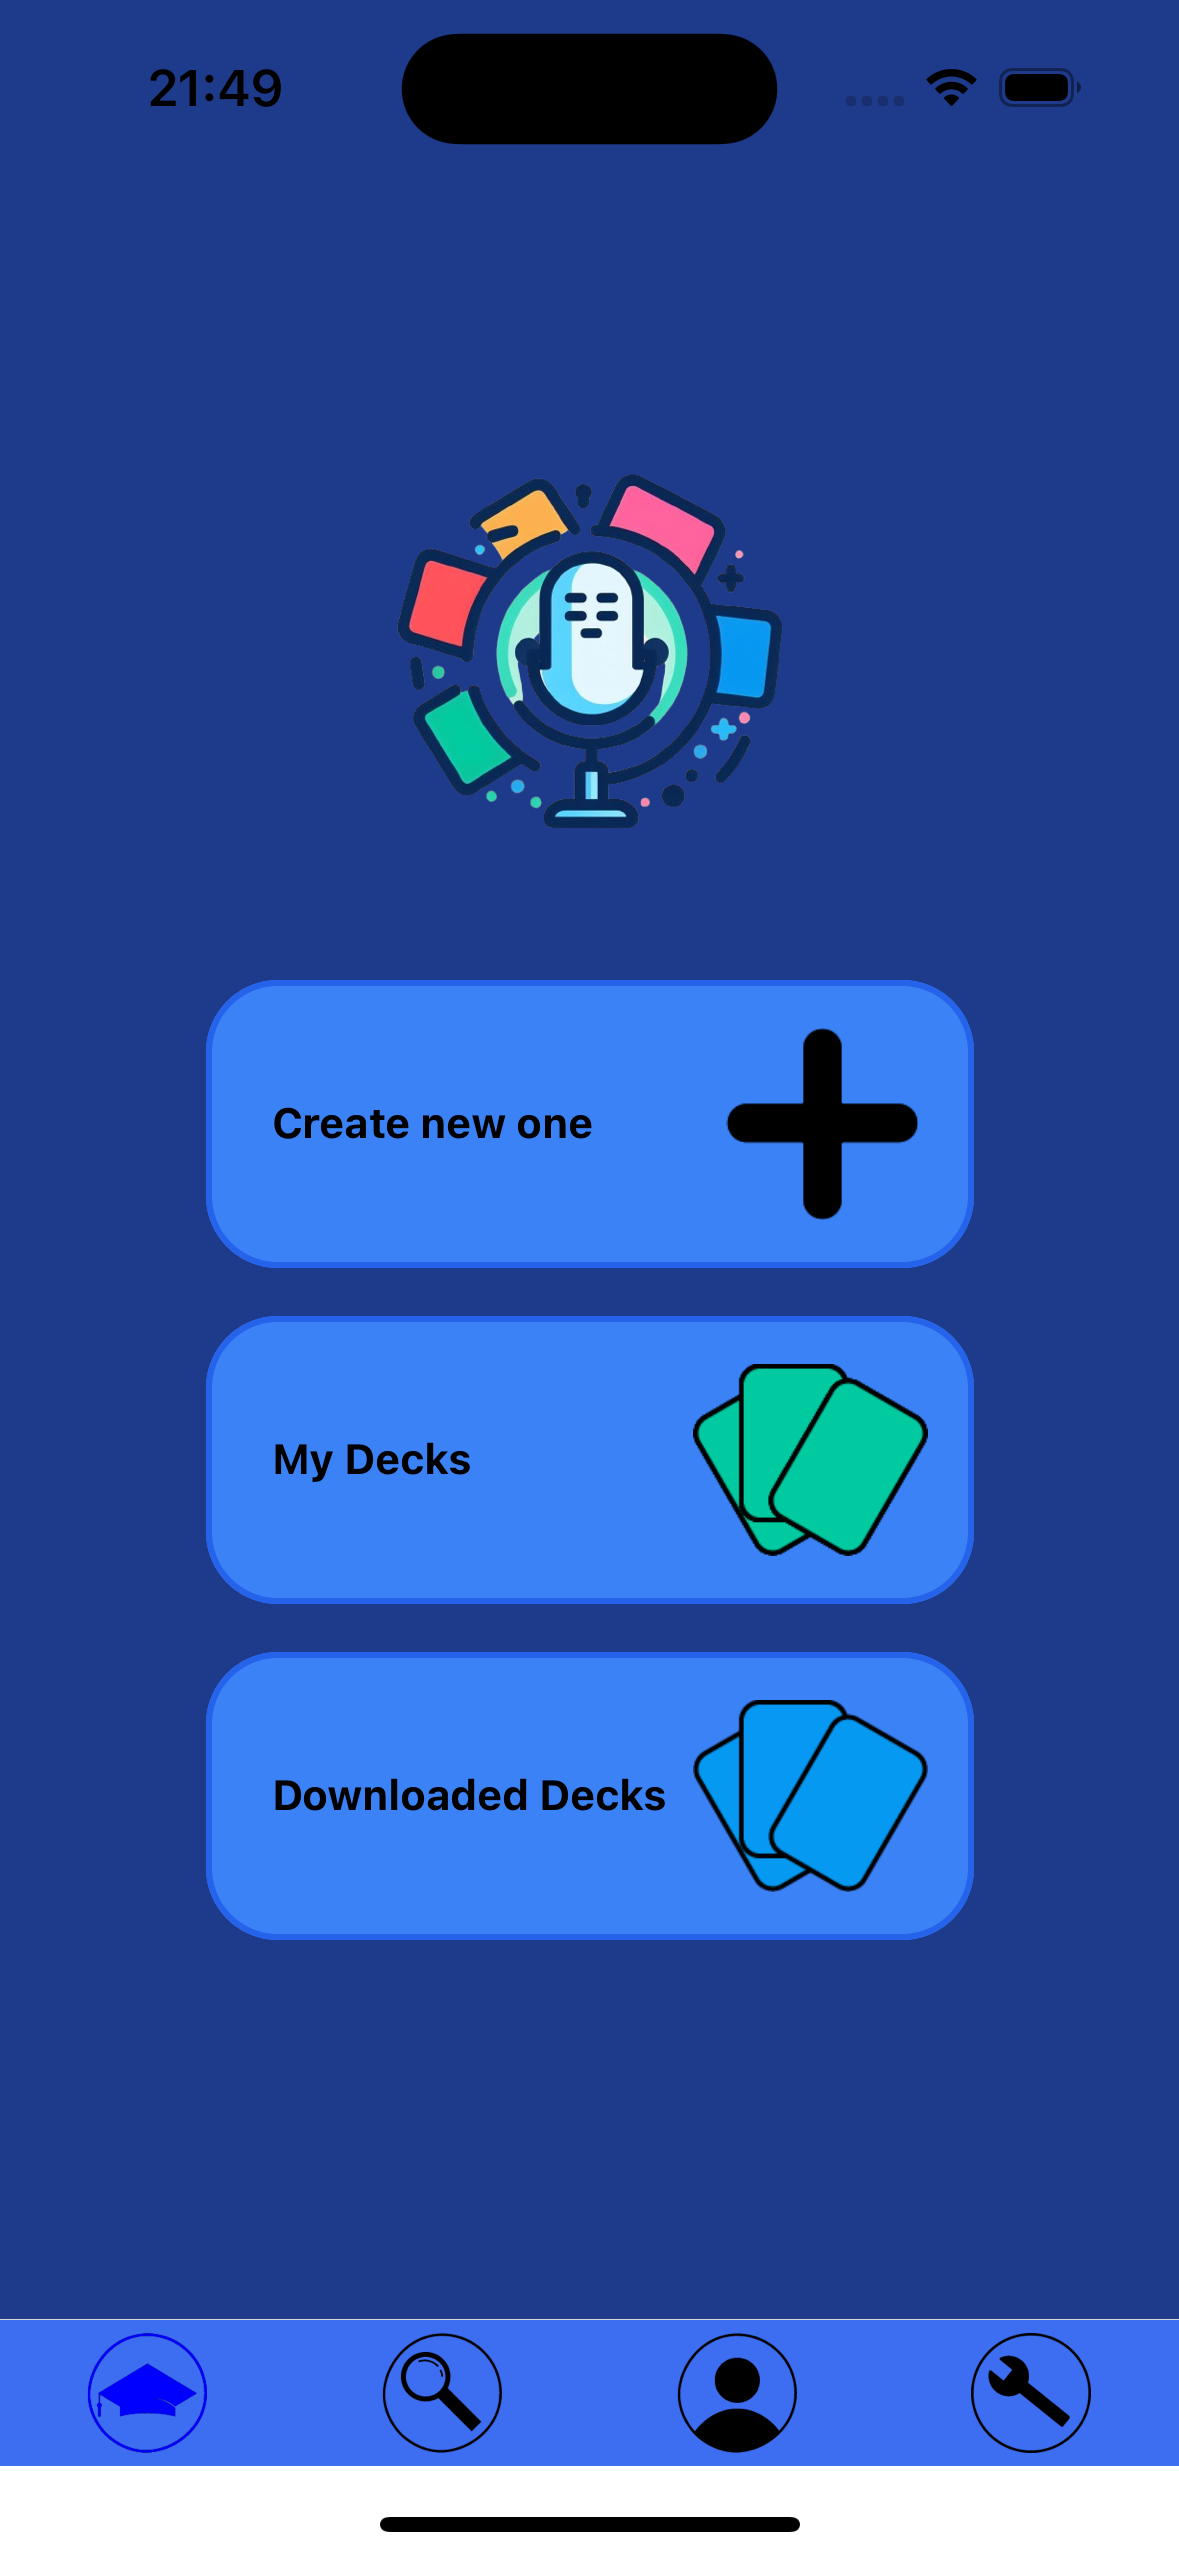
\includegraphics[width=0.5\textwidth]{chapters/chapter_10/images_mobile/dark_mode}
    \caption{Ekran domowy po przełączeniu na “Dark mode”.}
    \label{img:dark_mode}
\end{figure}